%%% File encoding: UTF-8
%%% äöüÄÖÜß  <-- keine deutschen Umlaute hier? UTF-faehigen Editor verwenden!

\documentclass[master,german]{hgbthesis}
% Zulässige Class Options: 
%   Typ der Arbeit: diplom, master (default), bachelor, praktikum 
%   Hauptsprache: german (default), english
%%%----------------------------------------------------------

%\overfullrule=5pt %use to show full boxes

\RequirePackage[utf8]{inputenc}		% Bei der Verw. von lualatex oder xelatex entfernen!

\graphicspath{{images/}}    % Abbildungsverzeichnis
\logofile{logo}				% Name des Logo-PDFs in images/ (\logofile{}, wenn kein Logo gewünscht)
\bibliography{literatur}  	% Name der Biblatex-Literaturdatei (.bib)

%%%----------------------------------------------------------
% Angaben für die Titelei (Titelseite, Erklärung etc.)
%%%----------------------------------------------------------

%%% Einträge für ALLE Arbeiten: -----------------------------
\title{Serverlose und verteilte Softwarearchitektur in einer Microservice-Umgebung (V5)}
\author{Philipp Haider}
\studiengang{Software Engineering}
\studienort{Hagenberg}
\abgabedatum{2017}{07}{07}	% {YYYY}{MM}{DD}

%%% Zusätzlich für eine Bachelorarbeit: ---------------------
\nummer{1510454013}   % Stud-ID, z.B. 1310238045-A  
% (A = 1. Bachelorarbeit)
\semester{Sommersemester 2017} 
%\gegenstand{Einführung in die Tiefere Problematik 1} 
\betreuer{Johann Heinzelreiter, FH-Prof. DI} % oder \betreuerin{..}

%%% Restriktive Lizenformel anstatt CC (nur für Typ master) -
%\strictlicense

%%%----------------------------------------------------------
\begin{document}
%%%----------------------------------------------------------

%%%----------------------------------------------------------
\frontmatter                    % Titelei (röm. Seitenzahlen)
%%%----------------------------------------------------------

\maketitle
\tableofcontents

\chapter{Kurzfassung}

Für die Realisierung von komplexen und skalierbaren Softwaresystemen ist ein Trend zur sogenannten Microservice"=Architektur, anstelle von monolithischen Architekturen zu beobachten. Bei diesem Architekturmuster handelt es sich um eine spezielle serviceorientierte Architektur, die aus tatsächlichen Anwendungsfällen von großen Internetfirmen hervorgegangen ist. In dieser Arbeit werden die Gründe für diesen Paradigmenwechsel gesucht und erläutert. Außerdem werden verschiedene Technologien für die erfolgreiche Umsetzung einer Microservice"=Architektur untersucht und miteinander in Verbindung gesetzt. Zu diesen Technologien zählen die Virtualisierung mit Containern, serverlose ereignisgesteuerte Funktionen und das Aktorenmodell. Auf Basis der genannten Konzepte gibt diese Arbeit Empfehlungen, für welche Szenarien der Microservices"=Ansatz überhaupt geeignet ist und wie dieser dann schlussendlich effektiv umgesetzt werden kann.		
\chapter{Abstract}

\begin{english} %switch to English language rules

The development of complex and scalable software systems has shifted from monolithic architectures towards the so called microservice architecture. This architectural pattern has evolved out of real world use cases of large internet corporations as a variant of the service-oriented architecture. First, this thesis provides a survey of the reasons behind this paradigm shift. Furthermore different technologies for successfully implementing microservices are shown and compared to each other. Among those technologies are containers for virtualization, serverless event-driven functions and the actor model. Based on the enumerated concepts this thesis provides recommendations to find suited applications for microservices and describes how to effectively apply this architectural style to complex software systems.

\end{english}
			

%%%----------------------------------------------------------
\mainmatter          % Hauptteil (ab hier arab. Seitenzahlen)
%%%----------------------------------------------------------

\chapter{Einleitung}

Das in dieser Arbeit verfolgte Ziel ist die Anwendbarkeit von verschiedenen Konzepten für Microservice"=Architekturen zu untersuchen und dabei die Unterschiede \bzw Gemeinsamkeiten herauszuarbeiten. In diesem Kapitel wird dafür zuerst der Stellenwert von Microservices hervorgehoben und anschließend die Struktur der Arbeit dargestellt.

\section{Motivation}

Moderne Anwendungen, vor allem im Web-Umfeld, unterliegen heutzutage immer größeren Anforderungen. Diese resultieren beispielsweise aus einer enormen Anzahl gleichzeitiger Benutzer, beträchtlichen Datenmengen oder dem erheblichen Zeitdruck im Wettbewerb mit Mitbewerbern. Um diesen Anforderungen gerecht zu werden, bedarf es oft sehr großer Entwicklungsmannschaften. Damit sinkt aber oft gleichzeitig die Effizienz, weil viele Abhängigkeiten zwischen Personen und Teams den gesamten Entwicklungsprozess verlangsamen. Unternehmen, die Anwendungen mit derartigen Anforderungen betreiben, haben die Ineffizienz dieses Ansatzes längst erkannt und versucht, diese Herausforderungen zu lösen. Daraus sind Vorgehensmodelle, Technologien und Architekturmuster entstanden, die heute unter dem Schirmbegriff "`Microservices"' zusammenfasst werden.

Statt der Entwicklung einer einzigen monolithischen Applikation hat sich in den letzten Jahren immer stärker das Architekturmuster Microservices etabliert. Dabei geht es um die Zerlegung eines komplexen Softwaresystems in unabhängige kleine Dienste. Diese sind voneinander isoliert und können nur über ein Netzwerk miteinander kommunizieren. Jeder Dienst soll dabei nur so groß sein, dass er genau eine Geschäftskompetenz des Unternehmens realisiert. An der Entwicklung sollen nur wenige Entwickler beteiligt sein. Durch diese Zerlegung wird ein viel effizienterer Entwicklungsprozess ermöglicht. Zusätzlich können bestimmte Teile des Systems unabhängig voneinander aktualisiert, ausgerollt und skaliert werden.

Für den Bedarf der Microservice"=Architektur sind verschiedene Entwicklungen verantwortlich. Zunächst hat das Internet über die globale Vernetzung einen riesigen Absatzmark für Software geschaffen. Anwendungen mit Millionen von Benutzern sind keine Seltenheit mehr. Auf technischer Seite sind wir mit einer Stagnation der Prozessorgeschwindigkeit konfrontiert. Prozessoren werden nicht mehr schneller, lediglich deren Anzahl steigt stetig. \Dah es sind verteilte Architekturen notwendig, die mehr, anstatt schnellerer Prozessoren ausnützen können. Gleichzeitig trägt auch der Konkurrenzkampf zwischen Unternehmen dazu bei, dass Entwicklungsprozesse agiler sowie die Einführungszeit neuer Produkte und Funktionen geringer werden. All diese Entwicklungen haben die Architektur heutiger Softwaresysteme wesentlich geprägt. Ein Resultat daraus ist die weitverbreitete Microservice"=Architektur, die der integrale Bestandteil dieser Arbeit ist.

\section{Gliederung und Struktur}

In dieser Arbeit werden verschiedene Konzepte und ihre Entstehungsgeschichte beschrieben. Sie gliedert sich in folgende Kapitel:

\begin{itemize}
	\item Kapitel~\ref{chap:microservices} gibt eine Einführung in die Microservice"=Architektur, grenzt sie zur monolithischen Softwarearchitektur ab und beschreibt mögliche Vorteile.
	\item Kapitel~\ref{chap:containers} beschreibt mit Containervirtualisierung eine leichtgewichtige Möglichkeit, Microservices sehr effizient bereitzustellen, ohne die Nachteile von klassischer Hypervisorvirtualisierung.
	\item Kapitel~\ref{chap:serverless} behandelt mit serverloser Programmierung einen noch leichtgewichtigeren Ansatz, ereignisgesteuerte Funktionen zur Verfügung zu stellen. 
	\item Kapitel~\ref{chap:actormodel} widmet sich mit Aktoren einem Modell für verteilte Programmierung, das viele Gemeinsamkeiten und Berührungspunkte mit der Microservice"=Architektur hat.
\end{itemize}

\section{Rahmen und Anwendungsbereiche}

In dieser Arbeit werden hauptsächlich Konzepte und Technologien betrachtet, die sich für die Implementierung von verteilbaren, skalierbaren und robusten Softwaresystemen eignen. Obwohl die Anforderungen an Software ständig steigen, benötigt nicht jedes System automatisch die genannten Eigenschaften in vollem Ausmaß. Wie im Laufe dieser Arbeit noch deutlich wird, sind viele Konzepte, gerade für kleine Systeme, teilweise sogar kontraproduktiv. Erst ab einer gewissen Komplexität können diese Konzepte ihren hohen Aufwand rechtfertigen. Es sollte daher immer genau abgewogen werden, ob sich die Verwendung eines bestimmten Ansatzes lohnt.

Die Microservice"=Architektur ist ein relativ abstraktes Modell, das nachträglich aus bestehenden Praktiken und Technologien geprägt wurde. Aus diesem Grund ist das Technologieumfeld um diese Architektur sehr breit, heterogen und schnelllebig. Diese Arbeit kann daher nur einen ausgewählten, aber dennoch repräsentativen Teil des gesamten Themenbereichs bearbeiten.

Das Kapitel über Containervirtualisierung konzentriert sich hauptsächlich auf die Verwendung von Containern für Microservices, den Unterschied zu Hypervisorvirtualisierung und mit Docker einer konkreten Containerplattform. Nur peripher wird auch Containerorchestrierung beschrieben. Hierbei handelt es sich um eine Art verteiltes Betriebssystem, dass zusätzliche nützliche Funktionen für die Verwaltung von Microservices bietet.

Als Stellvertreter für eine Fülle von serverlosen Plattformen steht in dieser Arbeit mit Azure Functions eine Technologie von Microsoft. Es geht aber keinesfalls um die Technologie selbst, sondern um die Grundidee einer serverlosen, ereignisgesteuerten Plattform, die verschiedene Standarddienste miteinander verbindet.

Den überwiegend aktuelleren Konzepten dieser Arbeit steht mit dem Aktorenmodell ein schon etwas älteres Konzept gegenüber. Daher ist es auch nicht verwunderlich, dass es hier die meisten unterschiedlichen Implementierungen gibt. Anhand von Erlang, der wohl bekanntesten und einer der ersten Implementierungen, werden die Grundlagen des Aktorenmodells erläutert. Darauf aufbauend folgen mit Orleans und Elixir zwei neuere Varianten.

Die in dieser Arbeit verwendeten Technologien sind also nur Stellvertreter für eine Menge von möglichen Alternativen. Es geht viel mehr um die Beziehung zwischen den dahinterliegenden Konzepten zu skalierbaren und robusten Softwaresystemen.
\chapter{Microservices}

Der Begriff Microservices stiftet derzeit noch große Verwirrung. Nicht nur weil er relativ neu ist, sondern auch weil er sehr breit gefächert ist und eine klare Abgrenzung kaum möglich ist. Im nachfolgenden Kapitel wird der Begriff Microservice ausführlich definiert, beschrieben und zu anderen Konzepten abgegrenzt.

\section{Was ist ein Microservice}

Hinter Microservices verbirgt sich keine konkrete Technologie oder ein Konzept das aktiv entwickelt wurde. Vielmehr ist es ein Sammelbegriff der nachträglich für über die Jahre entstandener Praktiken, Methoden und Technologien, im Umfeld von komplexen Softwaresystemen, eingeführt wurde. Am häufigsten ist mit Microservices die sogenannte Microservice Architektur gemeint. Charakteristisch für dieses Softwarearchitekturmuster ist die Zerlegung eines Softwaresystems in kleine, autonome Dienste, die über ein leichtgewichtiges Kommunikationsprotokoll miteinander kommunizieren. Die Fähigkeiten eines einzelnen Dienstes ist genau auf die Geschäftsanforderungen eines bestimmten Unternehmens oder Einsatzgebietes zugeschnitten \cite{FowlerMS}. Die Verwendung dieses Muster bringt aber neben technischen Einflüssen, meistens auch organisatorische Einflüsse mit sich. Beispielsweise auf die Teamstruktur, Verantwortung, Continuous Integration und Testen, um nur einige davon zu nennen. Daher können mit dem Begriff Microservices viele verschiedene Aspekte gemeint sein.

Um den rasanten Verbreitung der Microservice Architektur zu verstehen, ist es notwendig die klassische Architektur derartiger Systeme zu kennen. Dazu beschreibt der nächste Abschnitt den sogenannten monolithischen Ansatz und welche Probleme damit verbunden sind, die durch Microservices gelöst werden.

\subsection{Monolithischer Ansatz}

Mittlerweile haftet der monolithischen Softwarearchitektur ein negativer Ruf an. Jedoch zu unrecht, da dieser Ansatz seit Jahrzehnten  in vielen Bereichen der Softwareentwicklung sehr gut funktioniert. Im Java und .NET Umfeld war \bzw ist dieser Ansatz noch immer gängige Praxis. Dennoch wird er vielerorts von der Microservice Architektur abgelöst. Doch was macht eine Anwendung überhaupt zu einer monolithischen Anwendung?

Unter einer monolithischen Anwendung versteht man in der Softwareentwicklung eine Anwendung, in der verschiedene Geschäftsbereiche oder Funktionalitäten als eine einzige Anwendung zusammengeschlossen sind \cite{FowlerMS}. Intern kann die Applikation beispielsweise als Mehrschicht-Architektur organisiert sein. Üblich ist eine Drei-Schicht-Architektur mit folgenden Bestandteilen \cite{FowlerPEA}:

\begin{itemize}
	\item \textbf{Präsentationsschicht:} Hier ist jener Quelltext angesiedelt, der sich mit der Darstellung der Benutzerschnittstelle, \zB als Web- oder Desktop-Anwendung auseinandersetzt.
	\item \textbf{Geschäftslogikschicht:} Diese Schicht stellt den Kern der Anwendung dar. Sie enthält alle geschäftsrelevanten Funktionen.
	\item \textbf{Datenzugriffsschicht}: In dieser Schicht befindet sich die Funktionalität, die zum Zugriff auf externe Datenquellen, wie \zB einer relationalen Datenbank, notwendig ist.
\end{itemize}


In Abbildung \ref{fig:layered-architecture} ist der Aufbau einer monolithischen Anwendung mit Drei-Schicht-Architektur skizziert. Der Zugriff darf jeweils nur auf die direkt darunterliegende Schicht erfolgen. Innerhalb jeder Schicht ist eine Modularisierung in verschiedene Bereiche, die auf die Geschäftsfunktionen abgestimmt sind, sinnvoll.

\begin{figure}[!htb]
\centering
\minipage{0.5\textwidth}
  \centering
	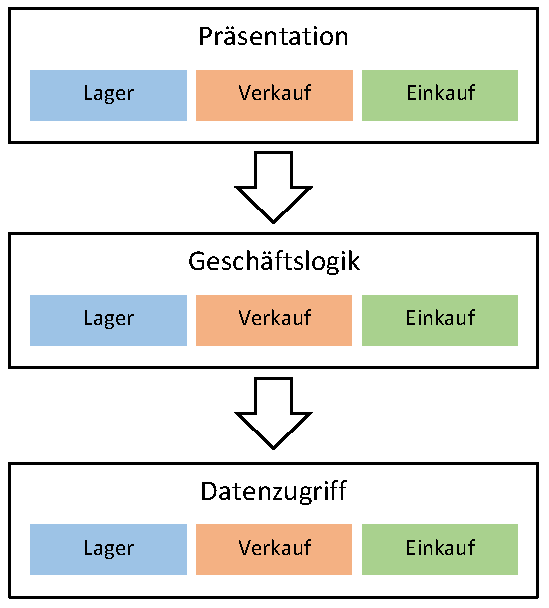
\includegraphics[width=0.8\linewidth]{layered-architecture}
	\caption{Drei-Schicht-Architektur}
	\label{fig:layered-architecture}
\endminipage
\minipage{0.5\textwidth}
  \centering
	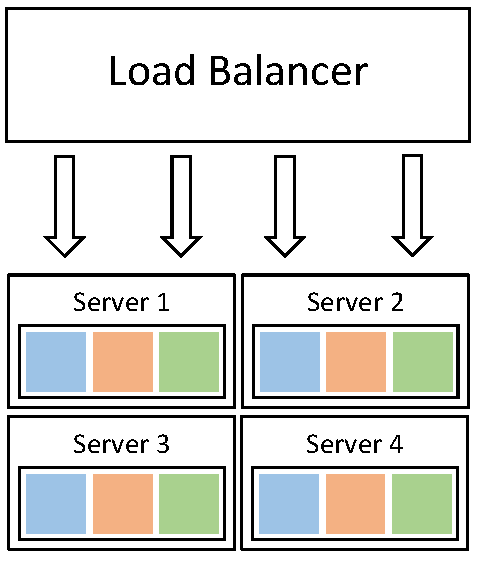
\includegraphics[width=0.76\linewidth]{monolith-scale}
	\caption{Skalieren einer monolithischen Anwendung}
	\label{fig:monolith-scale}
\endminipage
\end{figure}

\subsubsection{Nachteile und Schwierigkeiten}

Mit steigender Komplexität der Software kommen nach und nach Probleme zum Vorschein, die diesen Ansatz aufwändig oder sogar unpraktikabel machen. Eine der größten Herausforderungen bei der Entwicklung von Anwendungen mit globaler Reichweite ist die Skalierbarkeit. Die einzige Möglichkeit eine monolithische Anwendung zu skalieren, ist auf mehreren Servern jeweils eine Instanz der Anwendung zu installieren und über einen Load-Balancer zu verbinden. Abbildung \ref{fig:monolith-scale} zeigt wie ein solcher Aufbau aussehen kann. In vielen Einsatzgebieten ist dieser Ansatz aber nicht feingranular genug. Oft ist es sinnvoller, nur bestimmte Teile des Gesamtsystems zu skalieren.

Ein Monolith stößt aber nicht nur aus technischer Sicht auf Skalierbarkeitsprobleme, sondern auch aus organisatorischer Sicht. Alle Entwickler arbeiten zwangsläufig an der gleichen Codebasis, die dadurch enorme Größe annehmen kann. Kein einzelner Entwickler ist mehr in der Lage, die ganze Codebasis zu überblicken und zu beurteilen, welche Auswirkung eine Änderung haben kann. Das führt über kurz oder lang zur Verlangsamung der Entwicklungsgeschwindigkeit oder sogar zu völligem Stillstand.

Anforderungen an eine Software ändern sich häufig sehr rasch. Agile Softwareprozesse unterstützen dabei, die geänderten Anforderungen zeitnahe in die Software einfließen zu lassen. Für den Kunden \bzw Endbenutzer zählt nur die schnellstmögliche Umsetzung seiner neuen Anforderungen. In einer monolithischen Anwendung sind mehrere Geschäftsbereiche zusammengefasst. Somit muss die Anwendung immer als ganzes getestet und ausgerollt werden. Dadurch verlangsamt sich der gesamte Releasezyklus auf den langsamsten Teilbereich, obwohl vielleicht der geänderte Teilbereich schon längst fertiggestellt ist.

Hinter einer monolithischen Anwendung steht immer eine bestimmte Technologie oder eine Sammlung von mehreren Technologien, wie \zB Java EE oder ASP.NET. Somit müssen alle Teilbereiche der Anwendung auf die selben Technologien zurückgreifen. Für manche Teilbereiche könnte aber möglicherweise die Verwendung von alternativen Technologien und Speichersystemen große Vorteile bringen.

In diesem Abschnitt wurden einige der Hauptkritikpunkte am monolithischen Architekturmuster angeführt. Es mag den Anschein vermittelt haben, dass dieser Ansatz nicht mehr verwendet werden soll oder veraltet ist. Aber das ist so nicht der Fall. Viele Experten sind der Meinung, dass gerade am Anfang eines Projekts der monolithische Ansatz zu bevorzugen ist \cite{FowlerMolithFist}. Erst nachdem das Verständnis für die Domäne vorhanden ist und Anforderungen klarer sind, ist der fließende Übergang zu einer Microservice Architektur einfacher und sinnvoll. 

\section{Charakteristiken von Microservices}

Dieser Abschnitt beschreibt einige charakteristische Merkmale eines Microservices. Wie bereits erwähnt, gibt es keine eindeutige Definition eines Microservices. Daher ist es sinnvoller, allgemeine anerkannte Charakteristiken der Microservice Architektur zu betrachten.
 
\citeauthor{FowlerMS} identifizierte in \cite{FowlerMS} neun Charakteristiken von Microservices. Obwohl diese Liste bereits sehr exhaustiv ist, sind immer wieder sinnvolle Ergänzungen, wie in \cite{HorsdalMS} zu finden. Die nachfolgenden Abschnitte beschreiben eine repräsentative Auswahl dieser Charakteristiken.

\subsection{Organisation um Geschäftskompetenzen}

Normalerweise sind Softwareentwicklungsteams anhand ihrer technologischen Spezialisierung \zB in folgende Teams eingeteilt:

\begin{itemize}
	\item Front-End Entwickler
	\item Backend-End Entwickler
	\item Datenbank-Administratoren
	\item IT-Administratoren
\end{itemize}

Durch die Microservice Kultur hat sich aber eine andere Art der Teamstrukturierung etabliert. Für jede Geschäftskompetenz ist genau ein Team, welches intern aus einer kleinen Anzahl an den eingangs genannten Technologieexperten besteht, verantwortlich. Damit soll die Identifizierung und das Verantwortungsbewusstsein jedes einzelnen Teammitglieds für das von ihm entwickelte und betriebenen Dienstes stärken.

Was aber dennoch eine große Herausforderung bleibt, ist die Definition des Aufgabenbereichs eines einzelnen Teams. Die Identifikation und Abgrenzung der Geschäftskompetenzen eines Unternehmens ist eine sehr komplexe Aufgabe. Als Hilfsmittel lässt sich hier das \begin{english} Single-Responsibility-Principle\end{english} heranziehen \cite{MartinAgile}: 

\begin{english}
\begin{quote}
  \textit{A class should have only one reason to change.}
\end{quote}
\end{english}

Das aus der objektorientierten Programmierung bekannte Entwurfsprinzip kann auch im Kontext von Microservices angewandt werden. Es erweitert diesen Grundsatz von der Klassen-Ebene auf die Dienst-Ebene. Das heißt, jeder Dienst soll genau eine Fähigkeit realisieren. Damit ist sichergestellt, dass geänderte Geschäftsanforderungen so wenig wie möglich andere Microservices beeinflussen.

\subsection{Modularisierung durch Dienste}
\label{subsec:Componentization}

Seit Jahrzehnten strebt die Softwareentwicklungsbranche danach, komplexe Softwaresysteme einfach durch die Integration verschiedener Komponenten realisieren zu können. Durch dieses jahrelange bestreben und unterschiedlichste Ansätze ist leider auch der Begriff Komponente sehr überstrapaziert und hat dementsprechend viele unterschiedliche Bedeutungen. Beispielsweise in der objektorientierten Programmierung, kann eine Klasse als Komponente betrachtet werden. Darüber hinaus gibt es noch viele weitere Bedeutungen.

Auch wenn die konkrete Umsetzung einer Komponente sehr vielfältig sein kann, haben alle Arten die selben Ziele:

\begin{itemize}
	\item \textbf{Austauschbarkeit:} Es soll möglich sein, eine Komponente durch eine andere zu ersetzen. 
	\item \textbf{Wiederverwendbarkeit:} Eine entwickelte Komponente soll auch in anderen Systemen wiederverwendet werden können.
	\item \textbf{Aktualisierbarkeit:} Durch die Austauschbarkeit ist es automatisch möglich, eine Komponente durch eine neuere Version zu ersetzen, ohne den Rest der Anwendung zu beeinflussen.
\end{itemize}

Im Kontext der monolithischen Softwarearchitektur sind am häufigsten die Begriffe Modul oder Software-Bibliothek stellvertretend für den Begriff Komponente. Eine Anwendung besteht somit aus einer Menge von Modulen, die miteinander verbunden sind. Leider erfüllt dieser Ansatz die zuvor beschriebenen gewünschten Eigenschaften der Komponenten-Orientierung nicht ganz zufriedenstellend. Abhängigkeiten zwischen den einzelnen Modulen oder bestimmte Voraussetzungen an das Laufzeitsystem der monolithischen Anwendung können es schnell verhindern, ein Modul zu aktualisieren. Somit sind die verwendeten Komponenten nicht völlig voneinander unabhängig, sondern haben versteckte Abhängigkeiten.

In einer Microservice-Architektur ist mit Komponente ein einzelner Dienst gemeint. Damit ist jede Komponente ein eigener Prozess, der über ein Kommunikationsprotokoll mit anderen Komponenten interagiert. Mit diesem Ansatz lassen sich die gewünschten Eigenschaften viel leichter realisieren.

\subsection{Dezentrale Datenverwaltung}

Eine monolithische Anwendung legt sehr häufig alle persistenten Daten in einer einzigen relationalen Datenbank ab. Jeder Programmteil greift einfach auf die benötigten Daten direkt zu. Dieser Ansatz ist in Abbildung \ref{fig:central-datastore} dargestellt. In einer Microservice Architektur ist dieser Ansatz nicht mehr empfehlenswert. Persistente Daten eines bestimmten Geschäftsbereichs sollen nur von einem einzigen Dienst verwaltet werden. Direkter Zugriff auf diese Daten durch andere Dienste führt zu unerwünschten Abhängigkeiten. Andere Dienste müssen Daten über die öffentliche Schnittstelle des zuständigen Microservices abfragen oder verändern.

\begin{figure}[h]
  \centering
	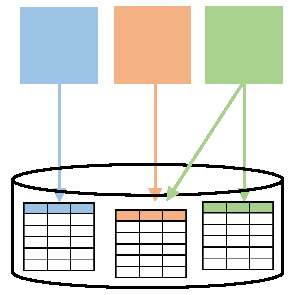
\includegraphics[width=0.3\textwidth]{central-datastore}
	\caption{Zentraler Datenspeicher}
	\label{fig:central-datastore}
\end{figure}

Wenn jeder Dienst wie in Abbildung \ref{fig:polyglot-persistnace} seinen eigenen Datenspeicher besitzt, kann für die Erfüllung seiner Aufgabe der optimale Speichermechanismus ausgewählt werden. Beispielsweise können Daten mit komplexen Beziehungen in einer Graphdatenbank abgelegt werden. Jedoch einfache Daten in einem schnellen Key-Value-Speicher.

\begin{figure}[h]
  \centering
	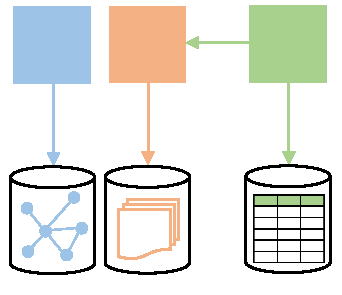
\includegraphics[width=0.3\textwidth]{polyglot-persistance}
	\caption{Polyglot Persistance}
	\label{fig:polyglot-persistnace}
\end{figure}

Auch eine monolithische Anwendung könnte Gebrauch von mehreren Datenbanken machen. Dieser Ansatz ist unter dem Namen Polyglot Persistence bekannt \cite{FowlerPP}. Aus teilweise sehr vielfältigen Gründen ist er aber selten anzutreffen. Nachfolgend nur ein kleiner Auszug:

\begin{itemize}
  \item Die IT-Strategie einiger Unternehmen sehen nur die Verwendung ganz bestimmter Datenbanken vor.
	\item Bereits getätigte Investitionen in bestehende Datenbanken müssen amortisiert werden.
	\item Angst vor dem Betrieb einer Datenbank für die noch nicht die notwendige Erfahrung aufgebaut wurde.
\end{itemize}

Für Systeme mit hohen Anforderungen an die Verfügbarkeit ist die Verwendung einer einzigen Datenbank nicht ausreichend. Denn eine einzige Datenbank stellt einen kritischen \textit{Single Point of Failure} dar.

\subsection{Automatisierung}

Für ein erfolgreiches System das aus Microservices besteht, ist ein hoher Grad an Automatisierung erforderlich. Durch die große Anzahl an Komponenten im System, muss die Anzahl an manuell erforderlichen Schritten sehr gering sein. Ansonsten ist der Aufwand für das Aktualisieren, Ausrollen, Testen und Überwachen viel zu groß.

Um von den Vorteilen der Microservice Architektur gegenüber einer monolithischen profitieren zu können, ist es unabdingbar, dass jeder Dienst einzeln ausgerollt werden kann. Denn nur damit sind die Entwicklungs- und Releasezyklen der einzelnen Dienste im Gesamtsystem voneinander unabhängig.

Wenn jeder Dienst einzeln ausgerollt werden kann, ist es auch möglich, unterschiedliche Versionen gleichzeitig auszurollen. Somit kann eine neue Version getestet werden und erst wenn diese Testphase erfolgreich abgeschlossen ist, der gesamte Datenverkehr auf diesen Dienst umgeleitet werden. Bei Problemen kann schnell der ursprüngliche Zustand wiederhergestellt werden. Insgesamt mindert ein derartiges Vorgehen das Risiko eines großen Big-Bang-Deployments.

Damit dieser Ansatz funktioniert, müssen die Dienste einige Anforderungen erfüllen. Jeder Dienst steht mit einigen anderen in Verbindung. Wenn nun eine neue Version eines Dienstes ausgerollt wird, muss dessen Schnittstelle abwärtskompatibel sein, da seine Konsumenten noch die alte Schnittstelle verwenden. Fehlertoleranz ist eine weitere wichtige Eigenschaft, da während eine neue Version ausgerollt wird, der Dienst kurzzeitig nicht verfügbar sein kann.

\subsection{Größe}

Wie der Name bereits suggeriert, soll ein Microservice klein sein. Das sollte schon durch die Anwendung des \textit{Single-Responsibility} Prinzips aus Abschnitt \ref{subsec:Componentization} gegeben werden. Wie groß ein Dienst genau sein soll, lässt sich aber aus vielen Gründen schwer festlegen. Die Anzahl der Quelltextzeilen ist ein schlechtes Maß für die Größe, da sie je nach Programmiersprache stark variiert. Schon aussagekräftiger ist die benötigte Zeitdauer für die Entwicklung des Dienstes. Aber auch diese Kennzahl kann trügerisch sein. Beispielsweise kann die Verwendung von externen Bibliotheken eine große Zeitersparnis erzielen. Jedoch inkludiert der Service dann auch die Komplexität dieser Bibliothek.

Eine genaue domänen-unabhängige Größenangabe ist praktisch nicht möglich. Es kann lediglich ein grober Rahmen abgesteckt werden. Ein Microservice sollte eine Entwicklungszeit von mehreren Wochen nicht übersteigen.

Neben quantitativen Kennzahlen sind oft subjektive Kriterien erforderlich. Eine davon ist, dass ein einzelner Entwickler die gesamte Funktionalität eines Dienstes noch im Kopf behalten können muss. Sobald es keinen einzelnen Menschen mehr gibt, der alle Aspekte des Dienstes auf einmal überschauen kann, ist er auf jeden Fall zu groß. Meistens aber haben erfahrene Architekten und Entwickler ein sehr gutes Gefühl, ab welcher Größe ein Dienst zu groß ist.

\section{Vorteile}

Ein neuer Softwareentwicklungsansatz setzt sich nur dann durch, wenn er auch einen erkennbaren Mehrwert bietet. Dieser Abschnitt zeigt einige der Vorteile, die durch den intelligenten Einsatz einer Microservice Architektur entstehen können \cite{fowlerMSTradeOffs,newman2015building}.

Es ist wichtig zu verstehen, dass die Vorteile, die durch Microservices entstehen, erst ab einer gewissen Größe \bzw Komplexität des Gesamtsystems zum Tragen kommen. In einfachen Softwaresystemen steht Komplexität der Microservice Architektur in keinem angemessenen Verhältnis zu den Vorteilen \cite{fowlerMSPremium}.

\subsection{Heterogener Technologieeinsatz}

Beim monolithischen Ansatz sind die Technologieentscheidungen äußerst eingeschränkt \cite{fowlerMSTradeOffs}. Nachdem die Haupttechnologie festlegt ist, kann aus diesem Korsett nur noch geringfügig ausgebrochen werden. Aber nicht für alle Aufgaben muss der eingeschlagene Weg auch der optimale sein.

Hier kommt ein wesentlicher Vorteil von Microservices zum Tragen. Da jeder Dienst eine kleine autonome Komponente ist, sind für jeden Dienst unterschiedliche sinnvolle Technologieentscheidungen möglich. Selbst die Wahl des Speichermechanismus kann individuell erfolgen. Die eingesetzte Technologie kann beispielsweise von der Aufgabenstellung oder den Fähigkeiten der Teammitglieder abhängig gemacht werden. Damit werden die Technologieentscheidungen nicht mehr von zentraler Stelle gesteuert, sondern die Kompetenz in die einzelnen Teams verlagert.

Die Macht der freien Technologieauswahl ist aber mit Bedacht einzusetzen. Es kann für ein System auch kontraproduktiv sein, wenn zu viele Technologien eingesetzt werden, die womöglich noch nicht einmal ein stabiles Stadion erreicht haben. Daher macht die Definition von team-übergreifenden Richtlinien zur Technologieauswahl durchaus Sinn. Der entscheidende Vorteil gegenüber dem monolithischen Ansatz ist aber die Wahlfreiheit, auch nach dem Start der Entwicklung.

\subsection{Robustheit}

Durch den hohen Modularisierungsgrad in einer Microservice Architektur herrscht ein ganz anderes Verständnis bezüglich der Verfügbarkeit von einzelnen Komponenten, wie in einer monolithischen Architektur. In einer monolithischen Anwendung befinden sind nämlich alle Komponenten in einem einzelnen Prozess. Daher kann ein Entwickler davon ausgehen, dass alle Komponenten immer verfügbar sind. Nicht so in einer Microservice Architektur. Hier muss jederzeit davon ausgegangen werden, dass Dienste nur eingeschränkt oder gar nicht verfügbar sind.

Wenn eine monolithische Anwendung ausfällt, ist das ganze System nicht mehr verwendbar. Im Gegensatz dazu kann das Gesamtsystem trotz des Ausfalls eines oder mehrere Microservices, zumindest eingeschränkt, weiterlaufen.

\subsection{Einfaches Deployment}

Jedes Release einer großen monolithischen Anwendung stellt ein gewisses Risiko dar. Daher passieren solche Releases in eher großen Abständen. In einem agilen Umfeld sind derartige lange Releasezyklen nicht tragbar. Außerdem kann jede kleine Fehlfunktion das ganze Deployment zum Scheitern bringen.

Mit Microservices ist es möglich jeden Dienst einzeln auszurollen. Damit ist die Auswirkung aus Sicht des Gesamtsystems viel geringer. Wenn der Dienst nach dem Ausrollen einen Fehler aufweist, kann nur dieser eine Dienst auf den Ausgangszustand zurückgesetzt werden.

Auch die Abhängigkeiten zwischen den einzelnen Teams ist durch den Microservice Ansatz reduziert. Ein Team kann ihren Service um Funktionalität erweitern und sofort ausrollen. Andere Teams die diese Funktionalität verwenden wollen, können erst dann neu ausrollen wenn ihr Dienst stabil ist. Dafür ist es aber notwendig, dass alle Dienste ihre Schnittstellen stets Rückwärts-kompatibel halten.

Die in diesem Abschnitt beschriebenen Vorteile einer Microservices Architektur sind keinesfalls allumfassend. Je nach Einsatzgebiet kommen möglicherweise auch andere Vorteile stärker zum tragen als die hier angeführten. Um von den Vorteilen profitieren zu können, ist eine ordentliche Umsetzung dieses Architekturmusters aber unumgänglich. Denn ansonsten hat man zwar die gesamte Komplexität die Microservices mit sich bringen, jedoch nicht die gewünschten Vorteile.

\section{SOA}

Ein kontrovers diskutiertes Thema im Bezug auf Microservices ist die Beziehung zu Service-orientierter Architektur, kurz SOA. Das abstrakte Architekturmuster SOA wurde bereits 1996 in \cite{schulte1996service} beschrieben und hat sich seither ständig weiterentwickelt.

Auch bei SOA ist es schwer, eine genaue Definition zu geben. Grundsätzlich handelt es sich dabei um eine lose gekoppelte Softwarearchitektur, in der die Komponenten der Software in Form von autonomen Diensten, um die Geschäftsprozesse gestaltet werden \cite{soaRW}. Neben dieser einfachen informellen Definition hafteten sich über die Jahre immer neue Konzepte an den Begriff an. Mittlerweile verbinden viele Architekten konkrete Technologien mit dem eigentlich abstrakten Konzept. Sehr häufig zählen dazu Technologien, wie SOAP, WSDL, WS-* Protokolle oder auch Nachrichten-orientierte Middleware Lösungen, wie ESB \cite{fowlerGoTo}. Aus diesem Grund stößt dieses Muster oft auf Ablehnung, da fälschlicherweise viele komplexe Technologien damit in Verbindung gebracht werden.

\citeauthor{newman2015building} beschreibt in \cite{newman2015building} die Beziehung zwischen Microservices und SOA, wie die Beziehung zwischen Scrum und agiler Softwareentwicklung. Wie Scrum eine konkrete Form von agiler Softwareentwicklung ist, können auch Microservices als ein bestimmter Stil zur Implementierung von SOA gesehen werden. Da alle Konzepte einer Microservice Architektur auch in SOA enthalten sind, können Microservices als Teilmenge und Konkretisierung von SOA verstanden werden.

Oft wird SOA dafür kritisiert, viel zu abstrakt und breit gefächert zu sein. Es gibt viel zu wenig konkrete Hilfestellungen, beispielsweise für den Entwurf von Service-Grenzen oder die Bestimmung der Service-Größe. Microservices hingegen wurde für einen bereits existierenden Stil der Anwendungsentwicklung nachträglich geprägt. Bei SOA hingegen wurde zuerst das Konzept definiert.

\section{Zusammenfassung}

In diesem Abschnitt wurden Microservices als um Geschäftskompetenzen entworfene, lose gekoppelte und autonome Dienste in einer service-orientierten Architektur, definiert. Der Begriff Microservices dient als Sammelbegriff für viele Konzepte die sich um dieses Architekturmuster scharen. Im Gegensatz zu SOA, ist die Vorstellung was Microservices sind, viel genauer, obwohl auch Microservices immer noch viel Interpretationsspielraum offen lassen.

Monolithischen Anwendung bündeln sämtliche Funktionalität eines Systems in einem einzigen großen ausführbaren Prozess. Bei der Microservice Architektur stehen wichtige Funktionalitäten als eigenständiger Dienst zur Verfügung. Das ermöglicht großen Teams, die Arbeit an komplexen Aufgaben, ohne sich gegenseitig zu stören. Damit ist es jedem Team selbst überlassen, die optimalen Technologieentscheidungen zu treffen, den Releasezyklus des Dienstes zu bestimmen und den Dienst in robuster Art und Weise zu implementieren.

Den Vorteilen der Microservices Architektur steht aber eine nicht zu unterschätzende Komplexität gegenüber. Beispielsweise die Orchestrierung aller einzelnen Dienste zu einer Einheit stellt eine große Herausforderung dar. Außerdem fließt viel Arbeit in die saubere Definition der Schnittstellen zwischen den Diensten ein. Einfache Anpassungen können schnell ausarten, da sie mehrere Dienste betreffen können. 

Nichts desto trotz hat das Microservice Architekturmuster in vielen Einsatzgebieten seine Vorzüge. Am Beginn einer Microservice Architektur sollte eine ausführliche Aneignung des erforderlichen Domänenwissens stehen. Oft funktioniert das nur durch den Start der Entwicklung mit einer monolithischen Architektur. Das Ziel sollte eine evolutionäre Architektur sein. Eine monolithische Architektur kann mit steigenden Verständnis für die Servicegrenzen leicht in eine Microservice Architektur überführt werden.
\chapter{Container-Technologien}
\label{chap:containers}

Dieses Kapitel beschreibt mit der Betriebssystemvirtualisierung in Containern eine effektive Möglichkeit, Microservices mit allen Abhängigkeiten in eine Einheit zu verpacken und effizient zu betreiben. Die technischen Grundlagen und Voraussetzungen dafür existieren schon einige Jahre, doch erst eine Implementierung mit dem Namen \textit{Docker} brachte neuen Aufschwung in diese Art der Virtualisierung. Mittlerweile ist Docker eine allgegenwärtige Methode, Software aller Art zu verteilen und zu betreiben.

Eine Microservice"=Architektur ist nicht nur aus Softwareentwicklungssicht herausfordernd, sondern auch aus Infrastruktursicht. Jeder Microservice muss unabhängig ausgerollt und skaliert werden können. Nur so kann diese Architektur auch die in Abschnitt \ref{sec:ms-advantages} beschriebenen Vorteile entfalten. Im Unterschied zu Hardwarevirtualisierung bietet dieser Ansatz wesentlich kürzere Bereitstellungszeiten und eine effektivere Nutzung von Ressourcen.

Jeder Service hat bestimmte Voraussetzungen an seine Infrastrukturumgebung. Dazu zählen externe Bibliotheken, Konfigurationen und meistens eine Laufzeitumgebung, wie \zB Java, .NET oder Python. Nun gibt es drei Möglichkeiten, die Infrastruktur über den gesamten Lebenszyklus eines Service zu verwalten. Am schlechtesten ist die benötigte Konfiguration manuell vorzunehmen. Dadurch ist es schwierig, Änderungen nachzuvollziehen und zu testen. Besser ist es, die Abhängigkeiten auf einem Server mit \textit{Infrastructure-as-Code} zu installieren und laufend zu aktualisieren. Ein alternativer Ansatz ist, den Service mit seinen Abhängigkeiten und Konfigurationen in ein Betriebssystemabbild -- \textit{engl. Image} -- zu verpacken \cite[113]{newman2015building}. Anstelle einer ausführbaren Anwendung wird einfach ein vollständiges Abbild eines virtuellen Servers erstellt und verteilt. Im folgenden Abschnitt wird dieser Ansatz noch näher präzisiert und anschließend mit \mbox{Docker} eine Technologie vorgestellt, die genau auf dieser Idee aufsetzt.

\section{Unveränderbarer Server}
\label{sec:immutable-server}

Anstatt die Konfiguration eines Servers zu ändern, kann man ihn auch stoppen und einen neuen Server mit aktualisierter Konfiguration wieder starten. Was sich anfänglich sehr aufwändig und unsinnig anhört, ist heute aus gutem Grund gängige Praxis. Das Unternehmen Netflix beispielsweise, praktizierte diesen Ansatz bereits sehr früh \cite{NflxLegos}. Laut eigenen Angaben konnten sie dadurch die Reproduzierbarkeit und Stabilität ihres Softwareauslieferungsprozesses stark verbessern. Zurückzuführen ist das auf die Tatsache, dass die in der Testumgebung validierten Artefakte identisch zu den im Produktivsystem eingesetzten sind. Des Weiteren gibt es keine Möglichkeit, wie eine Konfigurationsänderung unabsichtlich in ein Produktivsystem gelangen kann, ohne dass diese durch eine Reihe von Tests validiert wurde. Unter einem unveränderbaren Server versteht man also eine Ressource, die niemals verändert, sondern nur durch eine aktualisierte Version ersetzt wird \cite{ImmutableServer}.

\section{Arten von Virtualisierung}

Vor dem Einstieg in Container"=Technologien lohnt sich ein genauerer Blick auf verschiedene Virtualisierungstechniken. Nur wer die Eigenschaften der verschieden Systeme kennt, kann objektiv entscheiden, in welcher Situation welche Technologie vorteilhaft ist. Daher bietet dieser Abschnitt eine Darstellung verschiedener Virtualisierungskonzepte.

Unter Virtualisierung versteht man die Illusion, mehrere virtuelle und voneinander unabhängige Server auf einem einzigen physischen System auszuführen. Zum einen ermöglicht das eine effektivere Nutzung von Ressourcen und zum anderen die Möglichkeit, Server per Software zu verwalten. Über die Jahre wurden viele verschiedene Arten von Virtualisierung entwickelt. \cite{VirtualizationBasics} und \cite{Smith:2005:AVM:1069588.1069632} geben eine mögliche Klassifizierung verschiedener Ansätze.
Nachfolgend sind nur diejenigen Arten beschrieben, die für den Kontext dieser Arbeit relevant sind.

\subsubsection{Vollständige Virtualisierung}

Bei der \textit{vollständigen Virtualisierung} ermöglicht der sogenannte Hypervisor den Gastbetriebssystemen den Zugriff auf die Hardware. Die Gastsysteme sind unveränderte Betriebssysteme, die keine Kenntnis darüber haben, dass sie virtualisiert sind. Für jeden Gast wird eine vollständige Hardwareumgebung simuliert. Dieser Ansatz schützt die Gastsysteme gegenseitig sehr effektiv. Er ist aber auch sehr aufwändig, da jedes Gastsystem ein vollständiges Betriebssystem benötigt.

\subsubsection{Paravirtualisierung}

Wenn das Gastsystem Kenntnis über die Virtualisierung hat, dann spricht man von \textit{Paravirtualisierung}. Das Gastsystem verwendet sogenannte Hypercalls, um direkt mit dem Hypervisor zu interagieren. Damit lässt sich zwar eine Performanzverbesserung erzielen, jedoch ist dafür ein adaptiertes Gastbetriebssystem erforderlich. Diese Art der Virtualisierung kommt \zB in der Microsoft Azure Cloud zum Einsatz \cite[30]{Krishnan10}. Dort wird das Gastbetriebssystem als aufgeklärt -- \textit{engl. enlightend} -- bezeichnet.

\subsubsection{Prozessorunterstützte vollständige Virtualisierung}

Für die \textit{prozessorunterstützte vollständige Virtualisierung} greift der Hypervisor auf spezielle Prozessorfunktionen zurück. Der Befehlssatz dieser Prozessoren ist für Virtualisierungsszenarien erweitert, um eine Geschwindigkeitssteigerung zu erzielen und die Aufgaben des Hypervisors zu erleichtern. Durch die damit erreichte Komplexitätsreduktion der Hypervisorimplementierung sind diese viel einfacher und robuster zu implementieren.

\subsubsection{Betriebssystemvirtualisierung}

Die \textit{Betriebssystemvirtualisierung} unterscheidet sich stark von den anderen Arten. Hier gibt es keinen Hypervisor und auch die Gastsysteme sind keine vollständigen Betriebssysteme. Stattdessen werden sogenannte Container innerhalb eines Betriebssystems virtualisiert. Weil diese Art nur ein tatsächliches Betriebssystem erfordert und dieses von allen Container genutzt wird, ist sie effizient und ressourcensparend. Eine wesentliche Einschränkung ist derzeit aber noch, dass Container und das Wirtsystem auf dem selben Betriebssystem basieren müssen.

\section{Isolation versus Effizienz}
\label{sec:isolation-vs-efficiencys}

Virtualisierung ist immer ein Kompromiss zwischen Effizienz und Isolation. Jede Art zieht die Grenzen zwischen diesen beiden Eigenschaften an einem anderen Punkt. Die Effizienz lässt sich einfach anhand quantitativer Kriterien, wie dem Durchsatz oder Latenzzeiten festmachen. Bei der Isolation gestaltet sich die Situation schwieriger. In \cite{Soltesz:2007:COS:1272996.1273025} werden dazu folgende Kriterien herangezogen:

\begin{itemize}
	\item \textit{Fehlerisolation} ist gegeben, wenn ein Fehler in einem Gastsystem kein anderes Gastsystem beeinflussen kann.
	\item \textit{Ressourcenisolation} stellt sicher, dass die vorhandenen Ressourcen gerecht \bzw kontrollierbar auf die Gastsysteme aufgeteilt werden.
	\item \textit{Sicherheitsisolation} beschränkt den Zugriff auf Ressourcen wie dem Dateisystem, dem virtuellen Speicheradressraum oder dem Netzwerk.
\end{itemize}

Hypervisor- oder gleichbedeutend Hardwarevirtualisierung bietet bessere Isolation als Betriebssystemvirtualisierung, ist aber wesentlich ineffizienter. In vielen Szenarien, wie einer Microservice"=Architektur, ist strenge Isolation nicht notwendig, sondern kann gegen Effizienz eingetauscht werden.

\section{Docker}

Die zur Zeit bekannteste Betriebssystemvirtualisierungssoftware ist Docker. Im Gegensatz zur Hardwarevirtualisierung wird auf die Emulation einer Hardwareumgebung verzichtet und stattdessen auf der Betriebssystemebene virtualisiert. Durch den Verzicht auf diese Indirektionsschicht ist dieser Ansatz wesentlich effizienter.

Im Gegensatz zu anderen Virtualisierungstechniken steht bei \mbox{Docker} die Auslieferung von Software im Vordergrund. Ähnlich wie eine Paketverwaltungssystem kann Docker eine zentrale Stelle für die Verteilung von Software sein. Zusammengefasst erleichtert Docker den Bezug, die Installation, den Betrieb und die Aktualisierung von Software. Alle diese Möglichkeiten sind wertvolle Hilfsmittel bei der Realisierung einer Microservice"=Architektur.

\subsection{Begriffserklärung}

Im Umfeld von Betriebssystemvirtualisierung und Docker gibt es einige wichtige Begriffe. In \cite{paper_ernst_containers} ist eine umfassende Taxonomie über die Konzepte und Bestandteile von Container-Technologien zu finden. Ein kleiner Ausschnitt daraus sind folgende grundlegenden Begriffe:

\begin{itemize}
	\item Ein \textit{Image} ist die Vorlage für einen Container.
	\item Das \textit{Dockerfile} ist eine textuelle Beschreibung eines Images. Aufgrund dieser Beschreibung wird schlussendlich das Image erstellt.
	\item Ein \textit{Container} ist eine Laufzeitinstanz eines Images. Es kann beliebig viele Container"=Instanzen von einem Image geben. Auf Prozessebene besteht ein Container aus einem oder mehreren Prozessen, die von anderen Container- oder Host"=Prozessen isoliert sind. Durch die Isolation wirkt es für die Prozesse eines Containers so, als hätten sie das Betriebssystem exklusiv zur Verfügung.
\end{itemize}

Der nächste Abschnitt beschreibt mit den zuvor definierten Begriffen den grundsätzlichen Aufbau von Docker. Darüber hinaus werden signifikante Unterschiede zu Hardwarevirtualisierung hervorgehoben.

\subsection{Docker"=Architektur}

Docker implementiert eine klassische Client"=Server"=Architektur. Der Serverteil wird als \textit{Docker"=Engine} oder \textit{Docker"=Deamon} bezeichnet. Er interagiert direkt mit dem Betriebssystem, das schlussendlich die tatsächliche Virtualisierung realisiert. Der Server bietet eine REST"=Schnittstelle an, über die Klienten unterschiedlichster Art mit ihm kommunizieren können, um \zB Images zu erstellen, Container zu starten oder zu stoppen.

Um ein Image zu erstellen, sendet der Klient die Beschreibung in Form des "`Dockerfile"' und die benötigten Dateien an den Server. Dieser erstellt ein Image, das auf Basis der Beschreibung konfiguriert und mit allen benötigten Abhängigkeiten ausgestattet ist. Ausgehend von einem Image kann der Klient beliebig viele Container starten. In Abbildung \ref{fig:docker-arch} ist dieser Ablauf noch einmal visuell dargestellt.

\begin{figure}[!hbt]%
\centering
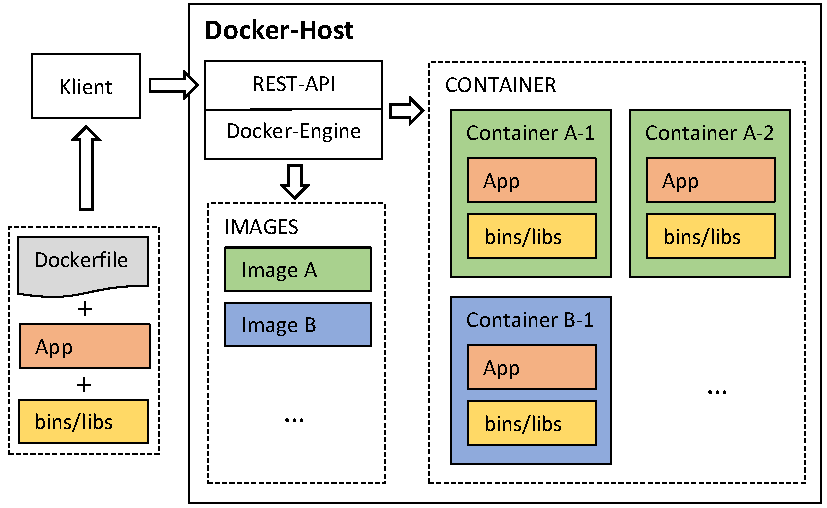
\includegraphics[width=\columnwidth]{docker-arch.pdf}%
\caption{Architektur von Docker}%
\label{fig:docker-arch}%
\end{figure}

Die genaue technische Umsetzung der Virtualisierung ist für jedes Betriebssystem spezifisch und übersteigt den Rahmen dieser Arbeit. Der folgende Abschnitt beschreibt nur einen komprimierten Überblick über einige grundlegende Konzepte im Betriebssystem Linux.

\subsection{Voraussetzungen für Betriebssystemvirtualisierung}
\label{subsec:docker-tech}

Ein Container ist nur auf der Betriebssystemebene von anderen Containern isoliert. Im Prinzip sind die in einem Container gestarteten Anwendungen  gewöhnliche Betriebssystemprozesse im Wirtsystem. Dennoch ist ein Container mehr ein virtuelles Betriebssystem als ein einfacher Prozess.

Die nachfolgenden Abschnitte basieren auf \cite{Merkel:2014:DLL:2600239.2600241}, sowie \cite{DBLP:journals/corr/Bui15} und beschreiben einige Betriebssystemkomponenten, die für die Virtualisierung verantwortlich sind.

\subsubsection{Namensräume}

\textit{Namensräume} bezeichnen im Betriebssystem \textit{Linux} eine Technologie, mit der Betriebssystemressourcen gruppiert und somit voneinander isoliert werden können. Dazu zählen beispielsweise Prozesse, Netzwerkverbindungen, das Dateisystem \usw Diese Technologie stellt somit die Isolation zwischen Containern und auch zum Wirtsystem sicher.

\subsubsection{Kontrollgruppen}

Wie Abschnitt \ref{sec:isolation-vs-efficiencys} schon dargestellt hat, ist eine faire Ressourcenaufteilung zwischen Containern sehr wichtig. Linux bietet dafür das Konzept der Kontrollgruppen. Damit kann der Ressourcenverbrauch von Containern überwacht und gegebenenfalls limitiert werden.

\subsubsection{Überlagerte Dateisysteme}

Durch die Verwendung eines speziellen Dateisystems kann Docker viele Daten zwischen Containern teilen und somit den Speicherplatz stark reduzieren. Die Grundidee ist, ein mehrschichtiges Dateisystem in eine einzige logische Sicht zu vereinen. Nur die oberste Schicht ist veränderbar. Alle anderen sind nicht beschreibbar und folglich unveränderbar. Eine Dateiänderung in einer höheren Schicht überdeckt die gleiche Datei einer niedrigeren Schicht.

Für beliebig viele Containerinstanzen ist somit nur eine einzige Kopie ihres Images auf der Festplatte notwendig. Mit dieser Technik ist eine enorme Speicherersparnis möglich, ohne die Isolation zu kompromittieren. Ein Betriebssystemabbild einer virtuellen Maschine mit Hardwarevirtualisierung ist um ein vielfaches größer und muss mehrfach abgespeichert werden. Je nach Betriebssystem gibt es verschiedene Implementierungen von überlagerten Dateisystemen. Zwei der bekanntesten Implementierungen sind das \textit{Advanced Multi-Layered Unification File\-system} und das \textit{OverlayFS}.

\subsection{Docker Beispiel}

Programm~\ref{prog:dockerfile} zeigt ein Beispiel für ein "`Dockerfile"', das ein Image mit einem Web"=Service erstellt. Im Basis"=Image ist bereits .NET Core -- eine Abhängigkeit des Web"=Services -- vorinstalliert. Im Prinzip erhält die Beschreibung alle notwendigen Schritte, um den Web"=Service auf einem leeren System zu installieren und zu konfigurieren. Die in Programm~\ref{prog:dockercommands} angeführten Kommandozeilenbefehle, erzeugen aus der Imagebeschreibung in Programm~\ref{prog:dockerfile} zuerst ein ausführbares Image, das anschließend gestartet wird.

\begin{program}[!hbt]
\caption{Beispiel für ein Dockerfile}
\label{prog:dockerfile}
\begin{DockerCode}
FROM microsoft/dotnet:1.1.1-runtime
COPY published app
WORKDIR app
ENV ASPNETCORE_URLS http://+:80 
EXPOSE 80
ENTRYPOINT [ "dotnet", "mywebapi.dll" ]
\end{DockerCode}
\end{program}

\begin{program}[!hbt]
\caption{Docker Kommandozeilenbefehle}
\label{prog:dockercommands}
\begin{GenericCode}
docker build -t sample-image .
docker run -d --rm -p 5000:80 sample-image
\end{GenericCode}
\end{program}

\section{Microsoft Windows Container}

Lange Zeit waren Container dem Betriebssystem Linux vorbehalten. Erst seit 2016 gibt es ein gleichwertiges Äquivalent für Windows Betriebssysteme~\cite{WinSerCont}. Windows Server 2016 ist das erste Windows"=Betriebssystem mit nativer Unterstützung für Betriebssystemvirtualisierung auf Basis von Docker. Auf vielen Servern kommt entweder das Betriebssystem Linux oder Windows zum Einsatz. Da Docker nun beide Systeme unterstützt, ist der potentielle Absatzmarkt sehr groß. Sowohl Linux- als auch Windows-Systeme halten sich an die selben Schnittstellen von Docker. Entwickler, die mit einem System vertraut sind, können ihr vorhandenes Wissen auch auf der anderen Plattform wiederverwenden.

In Linux sind Container, wie in Abschnitt~\ref{subsec:docker-tech} beschrieben, über Namensräume voneinander isoliert. Windows verwendet dasselbe Konzept, jedoch gibt es eine weitere Variante, die eine strengere Isolierung ermöglicht. Bei den sogenannten Hyper-V-Containern läuft jeder Container in einer eigenen leichtgewichtigen und für Container optimierten virtuellen Hyper-V"=Maschine \cite{WinConHyperV}. Der Verwender kann somit sehr leicht zwischen Effizienz und Isolation wählen.

Jedes Image basiert auf einem anderen Image. Nur sogenannte Basis-Images besitzen kein Eltern-Image. Im Prinzip sind Basis"=Images leere und auf das Minimum reduzierte Standardbetriebssysteme. Aufgrund der vielen verschiedenen Distributionen gibt es für Linux"=Container sehr viele Basis-Images. Für Windows-Container hingegen gibt es nur zwei. Das sogenannte Windows"=Server"=Core"=Image ist im Prinzip eine vollständige Windows-Server-2016 Installation, jedoch ohne Benutzeroberfläche. Die vielen gebotenen Möglichkeiten wirken sich aber enorm auf die Größe des Images aus. Eine schlankere Alternative ist das Nano"=Server"=Image. Diese abgespeckte Variante wurde speziell für Container entwickelt. Tabelle~\ref{tab:docker-image-size} zeigt den Speicherverbrauch von einigen ausgewählten Images und unterstreicht dabei die Leichtgewichtigkeit von Containern. Aufgrund der Wiederverwendbarkeit durch die geschachtelten Dateisysteme ist der Speicherbedarf aber nicht so problematisch wie bei virtuellen Maschinen.

\begin{table}[!hbt]
\caption{Image-Größe von ausgewählten Basis-Images (März 2017)}
\label{tab:docker-image-size}
\centering
\setlength{\tabcolsep}{5mm} % separator between columns
\def\arraystretch{1.25} % vertical stretch factor
\begin{tabular}{|r||c|c|c|}
\hline
\emph{Image} & \emph{Plattform} & \emph{Größe (entpackt)} \\
\hline
\hline
Ubuntu & Linux & 128 MB \\
\hline
Debian & Linux & 123 MB \\
\hline
CentOS & Linux & 193 MB \\
\hline
Alpine & Linux & 4 MB \\
\hline
Windows Server Core & Windows & 10.1 GB \\
\hline
Windows Nano Server & Windows & 1 GB \\
\hline
\end{tabular}
\end{table}

\section{Containerverwaltung}

Einen Container auf nur einem Server zu betreiben, ist eine triviale Aufgabe. Jedoch hunderte Container in einem Cluster mit mehreren Servern zu verwalten, ist ein ungleich komplexeres Unterfangen \cite{RussinovicContainers}. Aber dieses Szenario ist in einer Microservice"=Architektur eher die Regel eine die Ausnahme. Um diese Herausforderungen zu bewältigen, wurden viele Werkzeuge für die Cluster- und Containerverwaltung entwickelt. Eine essentielle Funktion von diesen Werkzeugen ist es, mehrere Container zu einer logischen Einheit zusammenzuschließen, sodass diese auch als Einheit verwaltet werden können. Des Weiteren bieten diese Werkzeuge eine Abstraktion der tatsächlichen Infrastruktur. So können mehrere Server zu einem Cluster verbunden und dieser als kohärente Plattform betrachtet werden. 

Der Begriff Orchestrierung beschreibt in der Softwareentwicklung die Kombination mehrere Dienste zu einer Komposition. Auch bei Containern spricht man von Containerorchestrierung, wenn mehrere Container zu einer Einheit zusammengeschlossen werden, um ihren Lebenszyklus gemeinsam zu verwalten. Ein Orchestrierer wird von vielen anderen Komponenten, wie \zB einem Scheduler oder einem Ressourcenmonitor unterstützt. 

Die Technologielandschaft rund um Containerverwaltung ist sehr breit und befindet sich noch stark im Aufbau. Eine umfassende Betrachtung dieses großen Bereichs würde den Rahmen dieser Arbeit sprengen. Dennoch ist es für eine Arbeit wie diese, die sich mit dem Thema Microservices auseinandersetzt, unumgänglich, diesen wichtigen Teilbereich zu erwähnen. Daher werden nachfolgend zumindest einige grundlegende Aspekte von Containerorchestrierung im Bezug auf Microservices dargestellt, die sich hauptsächlich auf \cite{ContainerOrcaWars} beziehen. 

\subsection{Funktionalität}

Die Hauptaufgaben eines Containerorchestrierers sind Maschinenbelegungsplanung, Ressourcen- und Serviceverwaltung. All diese Funktionen ermöglichen eine Reihe nicht"=funktionaler Eigenschaften, wie Skalierbarkeit, Verfügbarkeit oder Portabilität von Containern. Die am Markt verfügbaren Produkte unterscheiden sich vom Funktionsumfang und der Umsetzung der einzelnen Funktion.

\subsubsection{Maschinenbelegungsplanung}

Ein Orchestrierer muss entscheiden, auf welchem Server eine oder mehrere Instanzen eines Containers erzeugt werden. Serverausfälle sollen automatisch erkannt und betroffene Container auf einem anderen Server neu gestartet werden. In manchen Fällen bieten sie auch eine Unterstützung bei der Aktualisierung von Containerversionen.

\subsubsection{Ressourcenverwaltung}

Alle Hardwareressourcen, die ein Container in Anspruch nehmen kann, müssen überwacht und limitiert werden. Grundsätzlich betrifft das den Prozessor und den Hauptspeicher, aber auch den persistenten Speicher und Netzwerkressourcen.

\subsubsection{Serviceverwaltung}

Mehrere Container werden zu einer einzigen Applikation zusammengefasst, um sie gemeinsam zu verwalten. Im Zuge dessen müssen auch Abhängigkeiten zwischen Containern berücksichtigt werden, um beispielsweise eine sinnvolle Startreihenfolge festzulegen. Damit schlussendlich eine Anwendung auch skalierbar und hoch verfügbar ist, sind Lastverteilungsmechanismen notwendig, die auch vom Orchestrierer verwaltet werden.

\subsection{Verteilte Betriebssysteme}

Ein Betriebssystem bietet Anwendungsprogrammen eine Schnittstelle zu den Systemressourcen eines Computers. Somit müssen sich Anwendungsprogramme nicht mit der tatsächlichen Interaktion mit einer konkreten Hardwarekomponente auseinandersetzen, sondern sie greifen auf die abstrakten Schnittstellen des Betriebssystems zurück. Auch Containerorchestrierungswerkzeuge können als eine Art Betriebssystem verstanden werden, jedoch in verteilter Form. Statt Anwendungsprogramme teilt ein Orchestrierungswerkzeug Container \bzw aus vielen Containern zusammengesetzte Anwendungen einem mit Containervirtualisierungssoftware ausgestatteten Rechner zu. Der Kern dieses Systems ist die Containervirtualisierungssoftware, die auf jedem der verteilten Rechner läuft und natürlich die Orchestrierungssoftware, mit den im vorherigen Abschnitt beschriebenen Funktionen. Die verteilten Rechner und ihr tatsächliches Host"=Betriebssystem stellen die Systemressourcen dar. In vielen Fällen werden auch diese Systemressourcen als virtuelle Rechner zur Verfügung gestellt. In Abbildung~\ref{fig:container-distributed-os} ist die Analogie zwischen Betriebssystemen und Containerorchestrierungswerkzeugen noch einmal dargestellt.

\begin{figure}[!hbt]%
\centering
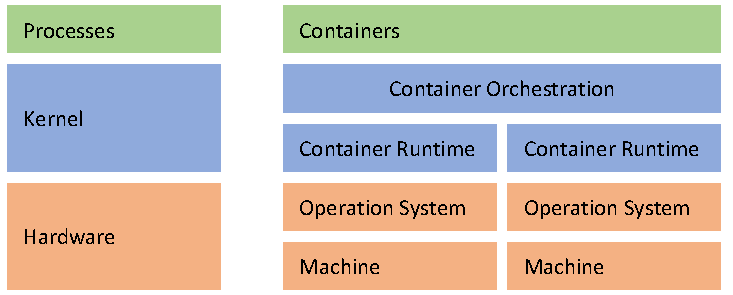
\includegraphics[width=.6\columnwidth]{container-distributed-os}%
\caption{Vergleich eines Betriebssystems (links) und eines "`verteilten Betriebssystems"' durch Containerorchestrierung \cite{ContainerOrcaWars}}%
\label{fig:container-distributed-os}%
\end{figure}

\subsection{Marktanalyse}

Studien, wie \cite{ContainerMarketGrowth}, sehen Container mit einer geschätzten jährlichen Wachstumsrate von bis zu 40 Prozent bis 2020 als einen der größten Zukunftsmärkte im Bereich Cloud"=Computing. Aufgrund dieser Zahlen ist es auch nicht verwunderlich, dass in diesem Bereich sehr viel investiert wird und dementsprechend viele Produkte auf den Markt kommen. 

Laut \cite{ContainerMarketReport} war Docker 2016 mit 94 Prozent das meist verwendete System für Containervirtualisierung. Bei der Containerorchestrierung jedoch sieht selbige Studie derzeit eine ausgeglichenere Marktaufteilung zwischen den Produkten \textit{Docker Swarm}, \textit{Kubernetes} und \textit{Apache Mesos}, wobei \textit{Kubernetes} die meisten Anteile dazugewinnen konnte.

\section{Zusammenfassung}

In diesem Kapitel wurde Betriebssystemvirtualisierung, im Speziellen mit Docker, als mögliche Plattform für Microservices vorgestellt. Ähnlich wie mit virtuellen Maschinen, ist es mit Docker möglich, eine Anwendung mit allen Abhängigkeiten zu verpacken, zu verteilen und zu betreiben. Jedoch ist Virtualisierung mit Containern viel effizienter und benötigt weniger Speicherplatz als Hardwarevirtualisierung.

Es wird immer seltener, dass die Software und die Konfiguration einer Server"=Infrastruktur laufend aktualisiert wird. Stattdessen werden diese langlebigen Server durch eine unveränderbare Infrastruktur ersetzt. Das heißt, anstatt einen Server zu aktualisieren, wird er durch einen neuen ersetzt. Unter einem Server ist in diesem Kontext meistens ein virtualisierter Server gemeint. Virtualisierungsplattformen wie Docker haben diesen Ansatz extrem effizient und robust gemacht.

Container alleine decken aber längst nicht alle Anforderungen an eine Infrastruktur für Microservices ab. Schnell sind Funktionen für die Skalierung, Verteilung, Aktualisierung oder die Überwachung von Containern notwendig. Für diese Aufgabe gibt es eine Menge von Containerorchestrierungswerkzeugen, die als eine Art verteiltes Betriebssystem über der Betriebssystemvirtualisierung agieren.

Unumstritten sind Container eines der zukunftsträchtigsten Technologiefelder der letzten Jahre, getrieben durch die DevOps"=Kultur und die Microservice"=Architektur. Vor allem im Bereich von Cloud"=Computing haben sie sehr großes Potenzial. Die Zukunft wird zeigen, ob und wie sich Container rund um bestehenden Plattform-as-a-Service-Angeboten platzieren können. 
\chapter{Serverlose Softwarearchitektur}

Die Bereitstellung und der Betrieb von Software"=Applikationen sind zwei oft unterschätze Kostenfaktoren. Viele technologische Entwicklungen der letzten Jahre, wie etwa Hardware"=Virtualisierung, Automatisierungswerkzeuge für Infrastruktur und Cloud"=Computing haben diese Kosten bereits stark reduziert. Dennoch ist der Einsatz einer selbst verwalteten Infrastruktur aufwändig und erfordert intensive Zusammenarbeit zwischen Entwicklern, IT"=Administratoren und Release"=Managern.

Vor der Bereitstellung einer monolithischen Software steht zuerst die Dimensionierung und Beschaffung der benötigten Hardware"=Infrastruktur durch die IT-Abteilung. Diese muss danach noch an die Bedürfnisse und Voraussetzungen der Software angepasst werden. Die Installation der eigentlichen Software ist oft ein manueller oder halb"=automatisierter Prozess. Das ist langsam und fehleranfällig, aber meistens akzeptabel, denn eine monolithische Software hat lange Release"=Zyklen und besteht aus einem einzigen Artefakt.

Die Verwendung des Microservice"=Architekturmusters verändertet diese Situation völlig. Mit diesem Szenario besteht ein einzelnes Softwaresystem aus einer Vielzahl von kleinen Diensten, die möglichst isoliert voneinander ausgeführt werden. Dazu ist eine sehr flexible und agile Bereitstellung der erforderlichen Ressourcen notwendig.

Mit \textit{Infrastructure-as-a-Service (IaaS)} bieten viele Cloud"=Computing"=Dienstleister die Möglichkeit, Server in wenigen Minuten bereitzustellen. Der Verwaltungsaufwand bleibt trotzdem relativ hoch, weil Betriebssystem"=Updates, IT"=Sicherheit, Netzwerkkonfiguration, \usw in der Verantwortung des Verwenders liegen.

Viele Applikationen benötigen kaum Kontrolle über die Umgebung in der sie ausgeführt werden. Für diesen Fall ist die Verwendung eines \textit{Platform-as-a-Service (PaaS)} Dienstes meistens vorteilhafter. Hier übernimmt der \textit{PaaS}-Betreiber die vollständige Verwaltung auf Hardware- und Betriebssystemebene, sodass der Verwender lediglich seine Anwendung im richtigen Format bereitstellen muss. Als Verwender hat man nur noch die Möglichkeit die Kapazität und Skalierbarkeitseigenschaften seiner Anwendung zu beeinflussen. Die genaue Umsetzung obliegt dem Anbieter dieser Dienstleistung.

Die Grundidee hinter \textit{Serverless Computing} ist dem Softwareentwickler eine Plattform für die Bereitstellung von Diensten zu bieten, ohne dass sich dieser um Server, deren Konfiguration oder Kapazitätsmanagement kümmern muss. Bei \textit{IaaS} und \textit{PaaS} ist das nicht oder nur zum Teil gegeben.

Wie viele Konzepte im Microservice"=Umfeld lässt sich auch serverlose Softwarearchitektur nur schwer abgrenzen. Im nächsten Abschnitt werden die zwei zur Zeit häufigsten Ausprägungsformen näher betrachtet.

\section{Arten serverloser Softwarearchitektur}

Serverlose Softwarearchitektur ist ein sehr junges Konzept, dessen weitere Zukunft noch offen ist. Derzeit haben sich aber schon zwei unterschiedliche Sichtweisen auf dieses Themengebiet herauskristallisiert \cite{ServerlessArchitectures}.

In der älteren Sichtweise beschreibt der Begriff \textit{serverlos} Applikationen die sehr stark auf vollständig verwaltete Dienste von Cloud"=Anbietern zurückgreifen. Darunter fallen beispielsweise verwaltete Datenbanken, Authentifizierungs- oder Benachrichtigungsdienste. Dieser Ansatz ersetzt also einen Großteil der Logik auf der Serverseite durch Dienste von Drittanbietern. Daher hat sich auch die Bezeichnung \textit{Backend-as-a-Service} dafür etabliert. Ein Teil der Applikationslogik muss aber dadurch vom Client übernommen werden. Mit JavaScript und verschiedenen Bibliotheken für die Erstellung von Benutzeroberflächen, lassen sich die dafür benötigten \textit{Rich-Applications} effizient realisieren.

Seit etwa 2014 hat sich die Sichtweise durch die Einführung des Dienstes \textit{AWS Lambda} durch \textit{Amazon} etwas geändert. Dieser Dienst erlaubt es, einfache Ereignis-gesteuerte Funktionen zu schreiben, die in der Cloud in einer zustandslosen Ausführungsumgebung vollständig verwaltet laufen. Die Artefakte die ein Entwickler erstellen muss sind einfache Skript"=Dateien die Funktionen mit der gewünschten Applikationslogik enthalten. Aus diesem Grund ist dieser Ansatz unter dem Namen \textit{Functions-as-a-Service (FaaS)} bekannt. Der folgenden Abschnitt beschäftigt sich intensiv mit dieser neuen Sichtweise auf Serverlose Softwarearchitektur.

\section{Functions-as-a-Service}

Im Grunde erlaubt es \textit{Functions-as-a-Service} kleine Aufgaben in Form von Funktionen zu programmieren und skalierbar, ohne weiteren Aufwand in der Cloud zu betreiben. Der Entwickler kann sich voll auf die Geschäftslogik seiner Applikation konzentrieren und muss sich kaum noch um Infrastrukturaufgaben kümmern.

Wie in den allermeisten Programmiersprachen auch, sind Funktionen in diesem Kontext eine relativ kleine Menge Quelltext die nach einer Aktivierung mit bestimmten Eingaben, Ausgaben produziert. Die Aktivierung erfolgt bei Programmiersprachen durch einen Funktionsaufruf. In \textit{FaaS} hingegen durch das Auftreten bestimmter Ereignisse die der Entwickler festlegen kann. Beispiele für derartige Ereignisse sind folgende:

\begin{itemize}
	\item Dem Hinzufügen eines Eintrags in einer Datenbank oder Warteschlange.
	\item Das Empfangen einer HTTP-Anfrage.
	\item Das Empfangen einer neue Nachricht in einer Nachrichtenorientierten Middleware.
	\item Das auftreten eines Zeitgesteuerten Ereignisses.
\end{itemize}

Eine Funktion ist nur dann sinnvoll, wenn sie auch Ausgaben oder zumindest Seiteneffekte produziert. In \textit{FaaS} können diese wieder sehr vielfältig sein. Meistens ist das Ergebnis die Interaktion mit einem anderen Cloud-Dienst wie \zB:

\begin{itemize}
	\item Dem Hinzufügen oder manipulieren von Daten in einer Datenbank.
	\item Das senden einer HTTP-Antwort.
	\item Das Versenden von Benachrichtigungen oder E-Mails.
\end{itemize}

Die folgenden Abschnitte beschreiben vielversprechende Anwendungsgebiete für \textit{FaaS}. Des weiteren werden die Konzepte \textit{FaaS} und \textit{PaaS} voneinander abgegrenzt.

\subsection{Anwendungsgebiete}

Für \textit{FaaS} gibt es in den verschiedensten Bereichen sinnvoll Anwendungsgebiete. Hauptsächlich werden sie aber für kleine und abgeschlossene Funktionalitäten herangezogen. Beispielsweise eignet es sich sehr gut für die Konvertierung und Validierung von Daten. Eine Funktion kann dabei auf ein bestimmtes Ereignis, \zB dem Hinzufügen eines Elements in einer Warteschlange warten, und danach die gewünschte Funktionalität ausführen. Das Ergebnis der Funktion kann \zB automatisch in eine Datenbank gespeichert oder an ein anderes System gesendet werden.

Microservice- und Cloud-Anwendungen verwenden oft eine große Anzahl von Cloud"=Komponenten wie, verschiedenen Datenspeichern, Warteschlangen und Nachrichtensysteme. Damit alle Einzelkomponenten in Summe ein funktionstüchtiges Gesamtsystem bilden, ist viel Logik für die Verbindung und Administration der Komponenten notwendig. Im Englischen wird diese Art von Logik häufig als \textit{Glue-Clode} bezeichnet, weil er die Einzelteile zum einem Ganzen "`zusammenklebt"'. Die Interaktion mit Cloud"=Komponenten ist also ein essentieller Bestandteil von und ist deswegen ein großer Einflussfaktor auf das Programmiermodell von \textit{FaaS}.

Der Erfolg der Microservice"=Architektur und \textit{FaaS} führte bereits zur Entstehung eines möglicherweise neuen Paradigmas: \textit{Nanoservices} \cite{infoqFaaS}. Bei Microservices stehen einzelne Geschäftsanforderungen im Vordergrund. Mit Nanoservice werden einzelne Geschäftsanforderungen noch weiter auf Funktionsebene heruntergebrochen. Ein Beispiel für einen Microservice könnte ein Dienst für die Abwicklung von Bestellungen sein, mit dem es möglich ist Bestellungen anzulegen, zu ändern oder zu verfolgen. Mit Nanoservices wäre jede einzelne dieser Funktionen ein eigener Dienst.

\textit{Amazon} beschreibt in \cite{AwsMultiTier} wie klassische Drei"=Schicht"=Architektur, \zB Web- oder Mobile"=Anwendungen, mit Serverlosen Technologie umgesetzt werden können . Darüber hinaus eignet sich \textit{FaaS} aber genau so gut für Microservice"=Architekturen. Die Einsatzgebiete sind daher sehr breit, was \textit{FaaS} zu einem mächtigen Werkzeug macht.

Viel Potential besteht in neuen Domänen wie \textit{Internet of Things}, \textit{Chat-Bots} oder \textit{DevOps} \cite{NewStackAzurePreview}. In diesen Bereichen ist die Nachfrage nach kleinen skalierbaren Programmen, die sich einfach entwickeln und betreiben lassen, sehr hoch. Durch die Einfachheit von \textit{FaaS} eignet es sich auch sehr gut für den Prototypenbau.

\subsection{Beziehung zu Platform-as-a-Service}

In vielen Bereichen überschneiden sich die Möglichkeiten von \textit{FaaS} mit denen anderer Technologien wie \zB \textit{PaaS}. Dieser Umstand ist nicht weiter verwunderlich, da \textit{FaaS} auf der Basis von \textit{PaaS} aufbaut. Der signifikanteste Unterschied ist die Ereignis-gesteuerte Funktionsweise von \textit{FaaS}. Funktionen werden nach dem Auftreten eines bestimmten Ereignis nur für die Dauer einer Aktivierung ausgeführt. Daher bezahlt der Verwender auch nur die Anzahl der Aufrufe und die Dauer der Ausführungszeit. Bei \textit{PaaS} ist meistens zumindest eine ständig laufende virtuelle Maschine erforderlich, die auf Ereignisse wart. Das Verursacht Kosten auch wenn die Maschine kaum oder gar nicht genutzt wird.

Skalierbarkeit ist in Cloud"-Computing ein essentieller Faktor. \textit{PaaS} bietet dafür die Möglichkeit, abhängig von Metriken wie Prozessorlast, die Anzahl der Instanzen auf denen die Anwendung ausgeführt wird, dynamisch zu erhöhen oder zu verringern. Dieser Ansatz erfordert bereits sehr wenig manuelles Eingreifen durch einen Entwickler oder Administrator. Aber \textit{FaaS} geht hier noch einen Schritt weiter und erfordert praktisch keine manuellen Handlungen um die Funktion skalierbar zu machen. Es ist die Aufgabe des Cloud"=Anbieters die Funktion automatisch zu skalieren. Weil die Funktionen zustandslos sind, kann man sie einfach beliebig oft parallel ausführen.

Die Verwendung von \textit{PaaS} schränkt Technologieentscheidungen stark ein, weil man sich auf eine konkrete Platform bindet. Bei \textit{FaaS} hingegen ist die Auswahl an möglichen Programmiersprachen sehr breit. Laufend fügen Cloud"=Anbieter neue Sprachen hinzu. Damit ist die Technologieabhängigkeit durch die Verwendung von \textit{FaaS} sehr viel geringer.

\subsection{Markt}

Alle namhaften Cloud"=Anbieter wie Amazon, Microsoft, IBM und Google haben bereits \textit{FaaS}"=Produkte in ihrem Angebot. Die nachfolgenden Abschnitte zeigen die Funktionsweise und Prinzipien anhand von \textit{Microsoft Azure Functions}, da diese Implementierung unter der MIT-Lizenz Open-Source verfügbar ist und somit tiefe Einblicke in die Umsetzung bietet. 

\textit{Amazon AWS Lambda} ist von allen Produkten am längsten am Markt und bietet den größten Funktionsumfang. Jedoch haben auch die anderen Anbieter das Potential und die Nachfrage von \textit{FaaS} erkannt und versuchen seither den Entwicklungsrückstand zu schließen.

Derzeit befindet sich dieses doch recht neue Thema noch stark im Wandel. Es ist sehr wahrscheinlich, dass sich einige Dinge in naher Zukunft verändern werden. Die Grundideen haben aber alle Anbieter ähnlich umgesetzt. Trotzdem unterscheiden sie sich in einzelnen Punkten:

\begin{itemize}
	\item Jeder Anbieter bietet unterschiedliche Programmiersprachen an. Es werden aber laufend neue Sprachen in die Produkte integriert.
	\item Auch wie das konkrete Skalierbarkeitsverhalten aussieht, muss beim jeweiligen Anbieter getestet werden.
	\item Meistens sind nur andere Dienste innerhalb des selben Cloud"=Anbieters mit \textit{FaaS} integriert. Dadurch kann sehr leicht eine starke Abhängigkeit zum gewählten Anbieter entstehen.
	\item Natürlich unterscheiden sich die einzelnen Angebote auch im Preis.
\end{itemize}

Derzeit investieren Cloud"=Anbieter sehr viel in die Entwicklung ihrer \textit{FaaS} Produkte. Das gibt einen Hinweis auf das große Potential dieser Technologie.

\section{Azure Functions}

Im März 2016 veröffentlichte die Firma \textit{Microsoft} eine Vorschauversion ihrer eigenen serverlosen Plattform mit dem Namen \textit{Azure Functions} \cite{AzFunIntro}. Nur ein halbes Jahr später folgte die erste offizielle Version \cite{AzFunGA}. \textit{Azure Functions} ist eine Erweiterung der ohnehin schon sehr umfangreichen \textit{Microsoft} Cloud"=Plattform. Diese Technologie eignet sich vor allem für die ereignisgesteuerte Verarbeitung und Transformation von Daten aus verschiedenen Datenquellen. Das deklarative Programmiermodell von \textit{Azure Functions} ermöglicht eine einfache Interaktion mit Daten- und Ereignisquellen. 

\textit{Microsoft} griff für die Implementierung von \textit{Azure Functions} auf folgende, schon länger in \textit{Microsoft Azure} enthaltene Dienste und Bibliotheken zurück \cite{AzFunJourney}:

\begin{itemize}
	\item \textit{App Service - Web App}
	\item \textit{App Service Plan}
	\item \textit{Site Control Manger (SCM)}
	\item \textit{Web Jobs}
	\item \textit{Web Jobs SDK}
\end{itemize}

Tatsächliche Neuentwicklungen waren folgende notwendig:

\begin{itemize}
	\item \textit{Web Jobs SDK Script}
	\item \textit{App Service - Function App}
	\item \textit{Dynamic Hosting Plan}
\end{itemize}

Die nachfolgenden Abschnitte geben einen Überblick hier aufgelisteten Bestandteile, die Entstehungsgeschichte und Anwendungsmöglichkeiten von \textit{Azure Functions}. Großteils beziehen sich die Grundlagen von \textit{App Services} und \textit{Web Jobs} auf \cite{AzWebEssentials4Devs}.

\subsection{Azure App Service}

\textit{App Service} ist in der \textit{Microsoft Azure} Cloud ein Oberbegriff für Services, die in die Kategorie \textit{Platform-as-a-Service} einzuordnen sind. Diese Services haben eine etwas konsequentere Interpretation von \textit{PaaS} als die älteren \textit{Cloud Services}. Bei einem \textit{App Service} übernimmt \textit{Microsoft} die Verwaltung der Infrastruktur, des Betriebssystems und der Laufzeitumgebungen. 

Ein \textit{App Service} ist einem sogenannten \textit{App Service Plan} zugeordnet. Dieser kann mehrere \textit{App Services} zusammenfassen, die auf einem oder mehreren Servern gemeinsam ausgeführt werden. Der \textit{App Service Plan} ist also eine abstrakte Infrastrukturbeschreibung, welche die Anzahl, Größe und das Skalierungsverhalten der virtuellen Maschinen festlegt. Daher wird er oft als \textit{Server Farm} bezeichnet.

Der nächste Abschnitt beschreibt mit \textit{Azure Web Apps} einen konkreten \textit{App Service}, der ein Grundbaustein hinter \textit{Azure Functions} ist.

\subsubsection{Azure Web App}

Eine \textit{Web App} ist in \textit{Microsoft Azure} der einfachste Weg um eine Web"=Anwendung bereitzustellen. Die virtuellen Maschinen des \textit{App Service Plan} in dem eine \textit{Web App} ausgeführt wird, sind bereits mit den gängigsten Webentwicklungsumgebungen ausgestattet. Damit lassen sich Web"=Anwendungen in unterschiedlichen Technologien gemeinsam betreiben. \textit{Web Apps} sind als eine Abstraktion eines Web"=Servers zu verstehen.

\subsection{Site Control Manager}

Die Funktionalität eines \textit{App Service} und somit auch einer \textit{Web App} ist mit Hilfe sogenannter \textit{Site Extensions} erweiterbar. Diese Erweiterungen werden im selben Kontext wie die eigentliche Web Anwendung ausgeführt. Der \textit{Site Control Manager} -- oft auch \textit{KUDU} genannt -- ist eine Erweiterung die bei jedem \textit{App Service} automatisch vorinstalliert ist. 

Anfänglich war die einzige Aufgabe des \textit{Site Control Manager} die Auslieferung des \textit{App Service} mittels Versionsverwaltungssystemen. Aber im Laufe der Zeit wurden weitere Funktionen ergänzt. Dazu zählt auch die Funktion \textit{Web Jobs}, welche die Abarbeitung von Hintergrundaufgaben ermöglicht. Für kleinere Aufgaben für die eine eigene virtuelle Maschine überdimensioniert wäre, sind \textit{Web Jobs} oft eine wirtschaftlichere Alternative.

\subsubsection{Web Jobs}

Als \textit{Web Job} eignen sich ausführbare Dateien oder unterstützte Skripte. Diese werden als eigener Prozess im Kontext eines \textit{App Service} entweder zeitgesteuert oder kontinuierlich ausgeführt. Damit können Hintergrundaufgaben überschüssige Kapazität ausnützen. Es kann aber auch zu negativen Effekten kommen, denn Hintergrundaufgaben können die Performanz der eigentlichen Web"=Anwendung für den Endbenutzer beeinflussen.

\subsection{Web Jobs SDK}

Die \textit{Web Jobs SDK} ist eine .NET"=Bibliothek für die Implementierung ereignisgesteuerter Hintergrundaufgaben. Das besondere daran ist das deklarative Programmiermodell, dass es erlaubt mit externen Datenquellen zu interagieren, ohne dafür extra Quelltext schreiben zu müssen \cite{WebJobsSdkBindingAttributes}.

Um vorab einen Einblick zu geben, zeigt Programm \ref{prog:webjobssdk} beispielhaft die Verwendung dieser Bibliothek. Der nächste Abschnitt enthält dann eine detailliertere Aufarbeitung der verwendeten Konzepte. Die folgende Aufzählung gibt eine Übersicht wichtiger Aspekte des Einführungsbeispiels:

\begin{itemize}
	\item Die Zeilen \textit{(1-5)} definieren eine Datenstruktur mit drei Attributen.
	\item Zeile \textit{(7)} startet die \textit{Web Jobs SDK} Laufzeitumgebung. Diese sucht per .NET Reflection nach kompatiblen Funktionen.
	\item Zeile \textit{(10)} definiert eine Funktion die ereignisgesteuert aufgerufen wird.
	\item Zeile \textit{(11)} definiert das Ereignis, das einen Funktionsaufruf auslöst. Hier wird die Funktion bei jedem neuen Eintrag in einer Warteschlangen aufgerufen und dessen Inhalt automatisch an den Funktionsparameter übergeben.
	\item Zeile \textit{(12)} definiert einen Ausgangsparameter. Wertzuweisungen an diesen Parameter werden automatisch in dem konfigurierten \textit{Blob Storage} gespeichert. Für den Pfad dieses Eintrags werden die aus dem Parameter in Zeile \textit{(11)} übergebenen Werte extrahiert.
	\item Zeile \textit{(13)} definiert einen weiteren Ausgangsparameter, der an eine andere Warteschlange weitergeleitet wird. Dieses Ereignis könnte wiederum einen anderen Funktionsaufruf auslösen. 
\end{itemize}

\begin{program}[!hbt]
\caption{Web Jobs SDK Beispiel}
\label{prog:webjobssdk}
\begin{CsCode}
  public class SensorData {
    public string SensorId { get; set; }
    public string Timestamp { get; set; }
    public double Value { get; set; }
  }
  class Program {
    static void Main() => new JobHost().RunAndBlock();
  }
  public class Functions {
    public static void ProcessSensorData(
      [QueueTrigger("sensorqueue")] SensorData sensorData,
      [Blob("values/{SensorId}/{Timestamp}")] out string sensorValue,
      [Queue("aggregationqueue")] out SensorData aggregationQueue) {
      sensorValue = sensorData.Value.ToString();
      aggregationQueue = sensorData;
    }
  }
\end{CsCode}
\end{program}

Obwohl die Funktion in Programm \ref{prog:webjobssdk} mit drei verschiedenen externen Datenquellen interagiert, enthält sie dafür fast keinen imperativen Quelltext, sondern lediglich eine deklarative Beschreibung in Form von Attributen. Die eigentliche Interaktion und das Warten auf Ereignisse ist die Aufgabe der \textit{Web Jobs SDK}. 

Eine \textit{Web Job} Anwendungen ist nichts anderes als eine gewöhnliche .NET Applikation mit einer Referenz auf die \textit{Web Jobs SDK}. Der nächste Abschnitt beschreibt wie statische Methoden einer \textit{Web Job} Anwendungen zu einem ereignisgesteuerten \textit{Web Job} werden.

Für viele Einsatzgebiete reicht dieses einfache, deklarative Programmiermodell aus. Es spricht aber nichts dagegen, die Interaktionslogik mit einer Datenquelle selbst im Funktionsrumpf zu implementieren. Das ist oft sogar notwendig, wenn der Funktionsumfang der deklarativen Variante nicht ausreicht. Der Grundgedanke ist jedoch derartigen repetitiven Standardquelltext durch deklarative Programmierung zu vermeiden.

\subsection{Bindungen}

Die zwei wesentlichen \textit{Web Job} Bindungen sind Trigger"=Bindungen und Nicht"=Trigger"=Bindungen. Erstere überwachen eine Ereignisquelle und lösen den Aufruf einer Job Funktion aus, wenn ein Ereignis auftritt. Zweitere binden Parameter einer Job Funktion an eine externe Datenquelle. Das kann sowohl zum Lesen, als auch zum Schreiben von Daten sein. Darum werden Nicht"=Trigger"=Bindungen in Eingangs- und Ausgangsbindungen eingeteilt. Jede Funktion muss genau eine Trigger"=Bindung haben, kann aber beliebig viele Nicht"=Trigger"=Bindungen enthalten.

Es gibt bereits eine Vielzahl vorhandener Bindungen. Entwickler können die Bibliothek aber auch mit selbst oder von Drittanbietern entwickelten Bindungen erweitern. Dazu muss man die wichtigsten dafür notwendigen Klassen kennen. Abbildung \ref{fig:webjobsclassdiag} zeigt den Bindungsmechanismus von Nicht"=Trigger"=Bindungen in einem stark vereinfachten Klassendiagramm.

\begin{figure}[!hbt]%
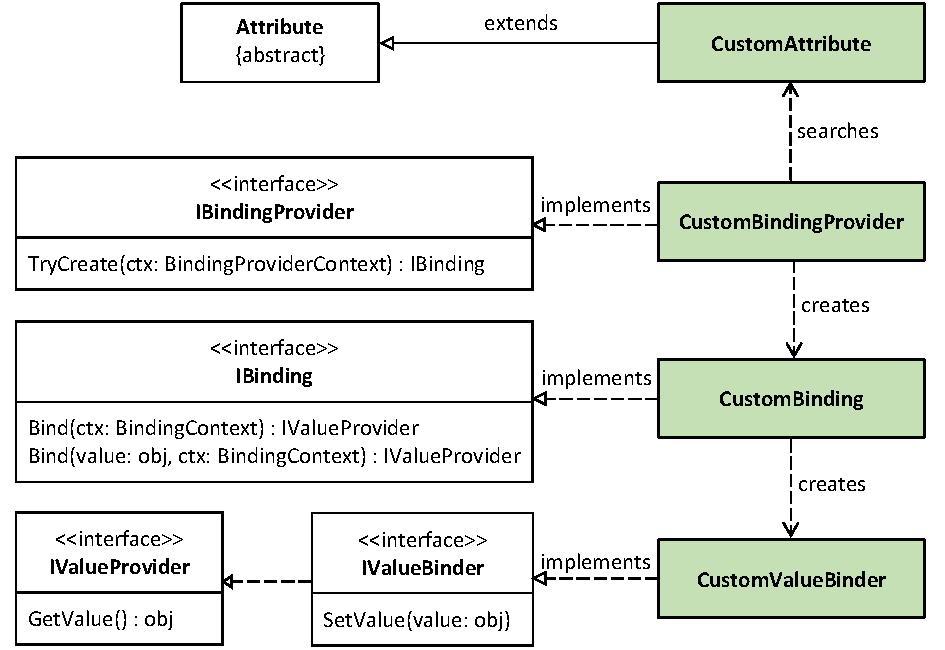
\includegraphics[width=\columnwidth]{webjob-ext-nontrigger-classdiag2}%
\caption{Web Jobs SDK Klassendiagramm (Nicht-Trigger-Bindung)}%
\label{fig:webjobsclassdiag}%
\end{figure}

Wie \cite{WebJobsSdkBindingProcess} beschreibt, ist der Bindungsprozess in zwei Phasen eingeteilt. Die nächsten Abschnitte beschreiben diese Phasen und geben somit auch Aufschluss darüber, wie die in Abbildung \ref{fig:webjobsclassdiag} skizzierten Klassen in Zusammenhang stehen.

\subsubsection{Startphase}

In der erste Phase beim Starten der Anwendung werden alle Funktionen auf ihre Tauglichkeit als \textit{Web Job} untersucht. Dieser Prozess umfasst folgende Schritte:

\begin{enumerate}
	\item Das Assembly der Anwendung wird nach allen Methoden in allen öffentlichen Klassen durchsucht.
	\item Für jeden Parameter einer Methode wird versucht eine Bindung zu erzeugen.
	\item Jeder registrierte \lstinline{I(Trigger)BindingProvider} bekommt die Möglichkeit eine Bindung über die Fabrikmethode \lstinline{TryCreate} zu erstellen. Diese Methode überprüft den Datentyp des Parameters und meistens die Existenz des Bindungs"=Attributs, welchess die Meta-Daten der Bindung beinhaltet. Sind die Voraussetzungen einer konkreten Bindung erfüllt, wird eine Bindung zurückgegeben.
	\item Wenn alle Parameter gebunden werden konnten, wird die Funktion im der \textit{Web Jobs} Laufzeitumgebung registriert.
	\item Für jede Trigger"=Binding wird zusätzlich die Überwachung der jeweiligen Ereignisquelle gestartet.
\end{enumerate}

\subsubsection{Laufzeitphase}

Nachdem alle Funktionen identifiziert wurden, beginnt die Laufzeitphase. In dieser Phase passiert die tatsächliche Bindung der Funktionsparameter. Dieser Ablauf lässt sich wie folgt zusammenfassen:
, wenn ein Funktionsaufruf durch ein Trigger"=Ereignis ausgelöst wurde.

\begin{enumerate}
	\item Ein Ereignis einer Trigger"=Bindung wird beobachtet und führt damit zur Ausführung der assoziierten Job Funktion.
	\item Für jeden gebundenen Parameter wird die \lstinline{BindAsync} Methode der zur Startphase festgelegten Bindung aufgerufen. In dieser passiert der eigentliche Interaktionsschritt mit einer externen Datenquelle, wie \zB dem Lesen von Daten aus einer Datenbank.
	\item Oft unterstützen Bindungen verschiedene Parametertypen, wie \zB \lstinline{String} oder \lstinline{Stream}. Die Bindung muss die tatsächlichen Werte auf den Datentyp der aufzurufenden Funktion konvertieren.
	\item Nachdem alle Parameter gebunden wurden, kann die eigentlich Funktion aufgerufen werden.
\end{enumerate}

\subsection{Web Jobs Script SDK}

Die \textit{Web Jobs Script SDK} ist das Herzstück von \textit{Azure Functions}. Es ist eine .NET Bibliothek, die eine interaktive Verwendung der sonst nur für .NET Applikationen geeigneten \textit{Web Jobs SDK} auch anderen Programmiersprachen zugänglich macht.

Die \textit{Web Jobs SDK} ist eine .NET Bibliothek und daher auch nur für .NET Anwendungen geeignet. Um die schon vorhandene Funktionalität auch für andere Sprachen und Platformen verfügbar zu machen, wurde die Bibliothek \textit{Web Jobs SDK Script} entwickelt.

- No Compilation step needed
- Simply change file - Runtime detects change
- Meta-Data in Attributes -> Meta-Data in Json file
- Folder structure - folder per function -> script files and config file


\subsection{Azure Function App}

Part of app services
Evolution of web jobs
Many languages
Serverless
Groups belonging functions together

- In Azure waren viele Bausteine für eine serverlose Platform bereits vorhanden (Web Jobs, Web Jobs SDK, ...)


\subsection{Verrechnungsmodell}

- GB/s
- Vergleich mit lasttest und dedicated service plan

\subsection{REST-Schnittstellen implementieren}

- Einfach REST implementieren
- Generisch?

\subsection{Kaltstart}

\subsection{Erweiterbarkeit}

\subsection{Zusammenfassung}

Ereignisgesteruert, interation
vieles bereits möglich
erst jetzt wirklich serverless
wann serverless und wann dedicated
kaltstart verbesserungen
lego baukasten

\section{Evolution der Anwendungsentwicklung}

Dieser Abschnitt bezieht sich weitestgehend auf \cite{Cock16EvoFunc} und \cite{Cock17ShrinkingMS} in denen der Autor Adrian \citeauthor{Cock16EvoFunc} die Evolution von monolithischer Software"=Architektur hin zu Microservices und weiter zu ereignisgesteuerten serverlosen Anwendungen beschreibt. Außerdem werden die dafür verantwortlichen technischen und organisatorischen Entwicklungen identifiziert.

Software"=Applikationen haben die Aufgabe Geschäftswerte -- \textit{engl. business value} -- zu generieren. Dazu müssen sie den Benutzern die enthaltene Geschäftslogik zugänglich machen. Eine Funktion kann erst Geschäftswerte erzeugen, wenn sie dem Benutzer tatsächlich zur Verfügung steht. Daher sollte die Minimierung der Zeit zwischen der Erstellung der Geschäftslogik und der tatsächlichen Verfügbarkeit für den Endbenutzer für Unternehmen an oberster Stelle stehen. \citeauthor{Cock16EvoFunc} beschreibt diesen Zusammenhang in folgender Formel:

\begin{center}
\textit{time to value = creation cost + delivery cost}
\end{center}

In der Vergangenheit war die Dauer zwischen der Erstellung und der Auslieferung einer neuen Funktion oft sehr lange. Aufgrund des hohen Aufwands und der zahlreichen Risiken eines neuen Releases, wurden Anwendungen nur in sehr großen Zeitabständen ausgeliefert. Zu dieser Zeit waren monolithischen Anwendung, in Verbindung mit einer oder wenigen zentralen relationalen Datenbanken, der effizienteste Weg Geschäftslogik bereitzustellen. Software"=Design war zu einem großen Teil durch Performanzbedenken dominierten. Die folgenden drei Abschnitte erläutern wie Hardware-Fortschritte, Auslieferungsautomatisierung und organisatorische Veränderungen, diese Probleme verringerten und somit den Weg für Microservices und serverlose Anwendungen ebneten.

\subsection{Automatisierung der Softwareauslieferung}

Vor einigen Jahren war die Bereitstellung von Software noch ein manueller Prozess. Die Beschaffung, Installation, Konfiguration und Aktualisierung von physischen Servern war ein wesentlicher Zeit und Kostenfaktor. Durch diese langsamen Vorgänge wurden nur selten, dafür eine große Menge Geschäftslogik, in einer neuen Softwareversion ausgerollt.

Eine zusätzliche Herausforderung stellte die Kapazitätsplanung dar. Viele Server wurden aufgrund der langsamen Änderungszyklen  vorsichtshalber sehr großzügig dimensioniert. Das führte wiederum zu einer unökonomischen Ressourcenauslastung.

Die Automatisierung von Infrastrukturaufgaben regte ein Überarbeitung festgefahrener Softwareauslieferungsprozesse aus. Werkzeuge wie \textit{Chef} und \textit{Puppet} erlaubten es erstmals, Skripte für die automatische Provisionierung und Konfiguration von Infrastrukturkomponeneten zu erstellen. Zu diesen Komponenten zählen Server, Betriebssystem, Netzwerk, Konfiguration, aber auch die Applikationssoftware selbst. Heute bezeichnet man diese Möglichkeiten als \textit{Infrastructure-as-Code}, weil sich Infrastruktur mittels Quelltext erstellen und manipulieren lässt. \cite[135]{Httermann:2012:DD:2380958}.

Wenn sich Infrasturktur wie Quelltext behandeln lässt, ist es naheliegend, dass auch Softwareentwickler an diesem Prozess teilnehmen. Die Infrastrukturprovisionierung und -verwaltung verlagerte sich allmählich von den IT"= in die Softwareentwicklungsabteilungen. IT"=Abteilungen und Cloud"=Anbieter stellten den Entwicklern nur noch Programmierschnittstellen -- sogenannte APIs -- zur Verfügung, mit denen sie selbst die Infrastruktur nach ihren Bedürfnissen erzeugen und verändern konnten. Diese Zeit- und Kostenreduktion bei der Softwareauslieferung ermöglichten häufigere Releases und viel kleinere Anwendungen. Schlussendlich war das eine der Voraussetzung für die Microservice"=Architektur. Die Auslieferung von Service veränderte sich von einem langsamen und risikoreichen Prozess in einen automatisierten.

Alle Anbieter serverloser Plattformen haben auf die Erfahrungen der Vergangenheit aufgebaut und Automatisierbarkeit von Anfang an berücksichtigt. Softwaresystemen mit einer großen Anzahl von Funktionen wären manuell schwer handhabbar. 

\subsection{Leistungsverbesserung der Hardware}

Erst der technologische Fortschritt der Netzwerkübertragungs- und Festplattengeschwindigkeiten haben den Weg für echte Service"=orientierte Architekturen geebnet. Obwohl die Ideen hinter SOA schon lange existieren, wurden sie aufgrund von Performanzengpässen gar nicht oder nur unzureichend umgesetzt.

Nachrichten-orientierte Systeme bedeuten immer einen gewissen Mehraufwand für die Übertragung und Kodierung der Nachrichten. Die Netzwerkgeschwindigkeit hat sich in den letzten Jahren um das zehn- bis hundertfache gesteigert \cite{IEEEBandwidth}. In der Ethernet Spezifikation \textit{IEEE 802.3-2015} sind Übertragungsraten bis zu 100 Gigabit pro Sekunde spezifiziert.

Eine weitere Erschwernis die für Nachrichtenübertragung waren schwergewichtige, oft XML-basierte, Kodierungsprotokolle wie \zB SOAP. Erst die Entwicklung von leichtgewichtigeren \bzw effizienteren Protokollen, in Kombination mit den um Größenordnungen schnelleren Netzwerkverbindungen, leiteten den Siegeszug von Nachrichten-orientierten Systemen ein.

Auch in der Speichertechnologie passierte durch die Ablösung von magnetischen Festplatten durch \textit{Solid-State} Festplatten ein weiterer essentieller Technologiefortschritt. Magnetische Festplatten sind ihren neuen Konkurrenten vor allem bei zufälligen Lesezugriffen deutlich unterlegen. Diese schlechten Zugriffszeiten waren der Grund für das Design großer monolithischer Datenbanken. Geschäftslogikfunktionen mussten viele Operation in einer Transaktion durchführen, um die langsamen Zugriffszeiten zu kaschieren.

Auf der Basis der sehr schnellen \textit{Solid-State} Festplatten wurden eine Menge neuer \textit{NoSQL} Datenbanken entwickelt. Diese wiederum haben die Dezentralisierung und die in Abschnitt \ref{subsec:polyglot-persistance} beschriebene polyglotte Persistenz der bis dato hauptsächlich monolithischen Applikation vorangetrieben.

Auch Funktionen in \textit{FaaS} machen intensiven Gebrauch von Nachrichtenübertragung und verschiedenen Datenspeichern. Im Grunde transformieren sie Daten, wann immer sie über eine Nachricht oder andere Ereignisse benachrichtigt werden.

\subsection{Organisatorische Veränderungen}

Abschnitt \ref{sec:business-capabilities} hat bereits beschrieben, dass Microservices eine Umstrukturierung der Entwicklungsteams zur folge hatte. Projekt- oder Technologie"=bezogene Strukturen wurde in Produkt-bezogene transformiert. Sehr große Teams wurden in viele kleine Teams zerlegt, um den hohen Koordinationsaufwand zu reduzieren. Jedes der Teams ist für den gesamten Lebenszyklus eines oder mehrerer Dienste verantwortlich. Diese Struktur erlaubte eine viel agileren Entwicklung und erfordert weniger definierte Prozesse.

\subsection{Von Microservices zu serverlosen Anwendungen}

Wenn man Microservices auf die Spitze treibt, erfüllt jeder Service nur noch eine einzige Aufgabe. Aufgrund der großen Anzahl von Services in einer Microservice"=Architektur, erfordert dieser Ansatz eine extrem effiziente Bereitstellung von Services. Selbst automatisch erstellte virtuelle Server und Container sind dafür ungeeignet. Für diese Anforderung ist \textit{Function-as-a-Service} eine gute Wahl, denn Funktionen lassen sich in Bruchteilen einer Sekunde ausrollen.

Viele Services werden nur selten oder sehr unregelmäßig genutzt. In diesen Szenarien ist es schwierig mit Containern oder virtuellen Maschinen die Kapazität zum richtigen Zeitpunkt bereitzustellen. Die Auslastung der Ressourcen ist in solchen Fällen meistens nicht optimal. \textit{Function-as-a-Service} ist sehr gut für volatile Lastaufkommen geeignet. Anstatt Rechenkapazität dezidiert zu reservieren, werden Funktionen erst bei Bedarf ausgerollt.

Funktionen enthalten beinahe ausschließlich Geschäftslogik. Es ist kaum Standard- oder Plattform"=Quelltext notwendig. Damit gelingt es Entwicklern oft binnen weniger Tage Funktionen zu entwickeln. Dabei verbinden sie einfach eine Funktion mit anderen Funktionen oder anderen Drittanbieter"=Diensten. Ein großer Vorteil von \textit{Function-as-a-Service} ist, dass die entwickelten Funktionen automatisch hoch skalierbar und hoch verfügbar sind.

Alle zuvor beschriebenen Eigenschaften machen \textit{FaaS} zu einer wertvollen Ergänzung der Microservice"=Architektur. Es gibt aber durchaus Szenarien in denen es nicht gut geeignet ist, beispielsweise wenn die Last sehr groß und vorhersehbar ist.

% INDEX

\iffalse
Serverless
- Intro
  - What
	- Why
	- Amazn
	- OSS
	- Competitors
- App Service Plan
- Kudu (Jobs, Deploy, Kinds, Scripts)
- Web Jobs SDK
  - Glue code
	- Locally / Dashboard
	- Core Arch
- Functions
  - Script Host Architecture
	- Dynamic Plan
	- Scaling
	- Threading
- Perf Benchmarks
- Pricing Comparison
\fi
\chapter{Aktoren}

In diesem Kapitel wird mit Aktoren ein Modell für nebenläufige Programmierung vorgestellt, dass ausschließlich auf asynchronen Nachrichtenaustausch basiert. Dieses Modell eignet sich vor allem für Systeme, in denen eine große Anzahl von Aufgaben gleichzeitigen ausgeführt wird. Zu diesen Szenarien zählen Systeme mit vielen Benutzer, gleichermaßen wie dem Internet der Dinge, das viele Geräte vernetzt.

Am Beginn dieses Kapitel werden die theoretischen Grundlagen des Aktorenmodells eingeführt. Anschließend wird mit der Sprache Erlang eine der ersten populären Implementierungen des Aktorenmodells präsentiert. Darauf aufbauend wird mit dem virtuellen Aktorenmodell eine mögliche Vereinfachung des Programmiermodells vorgestellt und diskutiert. Zum Abschluss dieses Kapitels wird noch die Beziehung des Aktorenmodells zur Microservice"=Architektur und anderen Technologien analysiert.

\section{Aktorenmodell}
\label{sec:actor-model}

Die ersten theoretischen Überlegungen des Aktorenmodells stellten \citeauthor{Hewitt:1973:UMA:1624775.1624804} bereits 1973 in \cite{Hewitt:1973:UMA:1624775.1624804} an. Hewitt beschreibt einen Aktor als fundamentale Recheneinheit die eine Möglichkeit benötigt \textit{Berechnungen} durchzuführen, einen \textit{Speicher} für Daten und die Fähigkeit zur \textit{Kommunikation} mit anderen Aktoren. Diese allgemeine Definition wird durch folgende drei Axiome ergänzt, die ein Aktor erfüllen muss:

\begin{itemize}
	\item Ein Aktor kann neue Aktoren erzeugen.
	\item Ein Aktor kann Nachrichten an andere Aktoren senden.
	\item Ein Aktoren kann sein Verhalten, dass bestimmt wie er auf die nächste Nachricht reagiert, ändern.
\end{itemize}

\noindent
Das Aktorenmodell ist nicht mit einem konkreten Programmierparadigma verbunden, sondern ein abstraktes Modell. Anschließend an diesen Abschnitt wird mit Erlang eine rein funktionale Implementierung vorgestellt und danach mit Project Orleans eine objektorientierte. Im Aktorenmodell finden sich viele Ideen aus der objektorientierten Programmierung, wie \zB Datenkapselung oder Nachrichtenaustausch wieder. Daher finden sich Entwickler mit einem Hintergrund in objektorientierter Programmierung oft sehr schnell mit der Funktionsweise des Aktorenmodells zurecht.

Ein einzelner Aktor hat nur begrenzte Möglihckeiten, daher kommen sie immer in ganzen Aktorsystemen vor. Da Aktoren eine sehr leichtgewichtige Einheit darstellen, können sehr viele Aktoren gleichzeitig in einem System existieren. Außerdem i das Erzeugen und Zerstören von Aktoren sehr effiziente Operationen. Aktoren bilden zur Laufzeit ein dynamisches Netzwerk, oder um es in der Sprache der Graphentheorie auszudrücken, einen gerichteten Graphen.

In sequentiellen Programmen wird Nebenläufigkeit meistens dadurch erreicht, dass mehrere Ausführungsstränge auf die selben Daten -- also den selben Speicherbereich -- zugreifen. Natürlich muss der Zugriff auf diese Daten geschützt und koordiniert werden, was diese Art der Programmierung schwierig und fehleranfällig macht. Nebenläufigkeit durch Aktoren, oder im allgemeinen durch Nachrichtenaustausch kann eine gute Alternative dazu sein. Aktoren besitzen keinerlei geteilten Speicher. Jede Information die sie benötigen müssen sie für sich selbst lokal speichern, oder als Teil einer Nachricht gesendet bekommen. Der Zustand eines Aktors ist somit für die Umwelt und damit auch für anderen Aktoren nicht sichtbar.

Die Verarbeitung der empfangen Nachrichten führt jeder Aktor sequentiell durch. Aber alle Aktoren können diesen Vorgang parallel durchführen. Gesamtheitlich gesehen ist dieses Modell also inhärent nebenläufig und somit gut skalierbar, auch wenn jeder Aktor für sich sequentiell ist. Je mehr Rechenkerne oder sogar Rechner zur Verfügung stehen, desto mehr Aktoren können gleichzeitig arbeiten.

Der Nachrichtenaustausch zwischen Aktoren erfolgt asynchron, \dh das Senden und das Empfangen der Nachricht ist entkoppelt. Eigentlich ist das Senden von Nachrichten asynchron, das Empfang jedoch ist für den Aktor eine synchrone \bzw blockierende Operation. Synchrone Kommunikation kann aber über Bestätigungsnachrichten nachgebildet werden. Bis zur tatsächlichen Verarbeitung einer Nachricht wird sie in einer Warteschlange zwischengespeichert. Manche Implementierungen des Aktorenmodells, darunter auch Erlang, unterstützen ein selektives Empfangen. Das bedeutet, dass nur bestimmte Nachrichten verarbeitet werden und andere in dieser Zeit in der Warteschlange verbleiben.

Das Aktorenmodell macht keine Annahmen darüber, ob es auf einem einzigen oder auf einen verteilten System angewendet wird. \Dah Programm die nach diesem Modell entwickelt sind, können ohne größere Änderung auf ein verteiltes System erweitert werden. Aktoren sind ohnehin nur über ihre Adressen angesprochen, die auch über Rechnergrenzen hinweg Bedeutung haben. Sie benötigen auch keinen gemeinsamen Speicherbereich, der in einem verteilten System ohnehin nicht existiert.

Obwohl Programme im Stile des Aktorenmodells in vielen Fällen einfacher sind als Systeme mit geteilten Speicher, schützt es dennoch nicht vor allen Herausforderungen der parallelen Programmierung. Probleme wie Deadlocks oder kritische Wettlaufsituation können durch falsche Anwendung dennoch entstehen. Aber später in diesem Kapitel genauer erläuterte Mechanismen wie Supervisorbäume und Zeitüberschreitungen helfen diese Probleme zu mindern.

\section{Erlang}
\label{sec:erlang}

Mit dem Ziel die Implementierung von hoch verfügbaren und verteilten Telekommunikationsanwendungen zu erleichtern, begann \citeauthor{Armstrong:1997:DE:258948.258967} 1985 die  Programmiersprache Erlang zu entwickeln~\cite{Armstrong:1997:DE:258948.258967}. In den Fokus seiner Bemühungen stellte er die Vereinfachung von nebenläufiger Programmierung. Die Begründung dahinter liegt darin, dass auch die reale Welt, die mit Software nachgebildet wird, inhärent nebenläufig ist. In jedem Augenblick passieren eine Unmenge an gleichzeitigen Ereignissen, die wir asynchron verarbeiten. Sequentielle Abläufe sind hier eher die Ausnahme. Trotzdem versuchen viele Programmiersprachen diese Tatsache zu ignorieren und stellen die sequentielle Hintereinanderausführung von Aktivitäten in den Vordergrund.

Um die Rolle der Nebenläufigkeit zu unterstreichen und Erlang von anderen Sprachen zu unterscheiden, bezeichnet Armstrong in \cite[19]{armstrong03} den Stil von Erlang als \textit{nebenläufigkeitsorientierte Programmierung}. Weitere wesentliche Einflussfaktor auf die Sprache sind die funktionale und teilweise die logische Programmierung, angelehnt an die Sprache Prolog.

Obwohl Erlang und das Aktorenmodell ein wenig in Vergessenheit geraten sind, erleben beiden derzeit wieder einen neuen Aufschwung. Das Interesse stieg vor allem wieder, nachdem die Kommunikationsplattform WhatsApp bekanntgab, dass sie mit ihren in Erlang entwickelten Plattform bis zu siebzig Millionen Nachrichten pro Sekunde verarbeiten~\cite{ErlangWhatsApp}.

\subsection{Einführung in die Sprache Erlang}

Dieser Abschnitt beinhaltet eine Einführung in die Syntax und Konzepte von Erlang, damit auch Leser ohne Vorkenntnisse in Erlang den Beispielen in diesem Kapitel folgen können. Die Sprache Erlang an sich ist wegen des minimalistischen Typsystems und der geringen Anzahl an Sprachfunktionen sehr einfach. Umfassendere Einführungen in Erlang geben die offizielle Dokumentation, \cite{Hebert:2013:LYE:2543986} und \cite{armstrong03}, auf denen auch ein wesentlicher Teil dieses Kapitels basiert.

\subsubsection{Typsystem}
\label{subsubsec:erlang-typesystem}

Die Sprache Erlang lässt sich als dynamisch und stark typisiert charakterisieren. Das sehr einfache Typsystem umfasst acht primitive und mit Tupel \bzw Listen zwei zusammengesetzte Datentypen, die nachfolgend noch erläutert werden.

In \cite{Marlow:1997:PSS:258948.258962} wurde versucht Erlang um ein statisches Typsystem zu erweitern, um Programmierfehler schon zur Übersetzungszeit zu identifizieren. Obwohl dieser Ansatz teilweise erfolgreich war, wurde er nicht weiter verfolgt, weil nicht alle Teile der Sprache typisiert werden konnten~\cite[14]{Armstrong:2007:HE:1238844.1238850}. Später wurde ein Werkzeug für leichtgewichtige statische Code"=Analyse mit dem Namen \textit{Dialyzer} entwickelt~\cite{ErlangWarStory}. Im Gegensatz zum dem in \cite{Marlow:1997:PSS:258948.258962} verfolgten Ansatz benötigt der Dializer keine zusätzlichen Typ"=Annotationen durch den Programmierer und erkennt dennoch die meisten Fehler die auch ein statisches Typsystem erkennen würde.

\subsubsection{Variablen}

Wie in vielen funktionalen Sprachen sind Variablen unveränderbar. \Dah es kann nur einmal ein Wert zugewiesen werden. In Erlang spricht man häufiger vom "`Binden"' einer Variable an einen Wert. Per Konvention beginnen alle Variablennamen mit einem Großbuchstaben. Programm~\ref{prog:erlang-vars} zeigt einige Beispiele für die Verwendung von Variablen.

\begin{program}[!hbt]
\caption{Verwendung von Variablen in Erlang}
\label{prog:erlang-vars}
\begin{ErlangCode}
Var1 = 1 + 2.
Var1 = Var1. % succeeds because left and right hand side are equal
Var2 = Var1 + 1. % succeeds and Var2 = 4.
Var1 = Var1 + 1. % fails because left and right side don't unify
\end{ErlangCode}
\end{program}

\subsubsection{Atome}

Atome bezeichnen in Erlang ein primitiven Datentyp, der wie ein Literal oder eine Konstante zu verstehen ist. Während Variablennamen immer mit einem Großbuchstaben beginnen, müssen Atome mit einem Kleinbuchstaben beginnen, damit sie unterscheidbar sind. In Programm~\ref{prog:erlang-atom} ist die Zuweisung eines Atoms an eine Variable gezeigt.

\begin{program}[!hbt]
\caption{Verwendung eines Atoms in Erlang}
\label{prog:erlang-atom}
\begin{ErlangCode}
Var3 = myatom.
\end{ErlangCode}
\end{program}

\subsubsection{Tupel und Listen}

Ein Tupel ist eine endliche Folge fixer Größe, die mehrere Elemente zu einem Verbund zusammenfasst. Die Anzahl der Elemente in einem Tupel ist endlich und nicht veränderbar. Neben Tupel besitzt Erlang auch einen Listentyp, der für eine beliebige Anzahl von Elementen aufnehmen kann. Im Gegensatz zu anderen Programmiersprachen müssen die Typen der Listenelemente nicht homogen sein. Tupel und Listen scheinen äußerlich sehr ähnliche Fähigkeiten zu haben. Generell gilt aber, dass Tupel für Datenstrukturen und Listen für Sequenzen von Elementen vorgesehen sind. Programm~\ref{prog:erlang-lists} zeigt einige Beispiele wie Listen deklariert werden können.

\begin{program}[!hbt]
\caption{Verwendung von Listen in Erlang}
\label{prog:erlang-lists}
\begin{ErlangCode}
Person1 = { alice, "Fake Street 42", 1234 }.
Person2 = { bob, "Main Avenue 1", 5678 }.
Person1 = { person, alice, "Fake Street 42", 1234 }. % mimics a class
List1 = [ 1, two, "three" ].
List2 = [ 1 | [2 | [ 3 | [] ] ] ].
List3 = [ Person1, Person2 ].
\end{ErlangCode}
\end{program}

\subsubsection{Module und Funktionen}

Module sind Dateien die mehrere logisch zusammengehörende Funktionen zu einer Einheit gruppieren. Das ermöglicht eine bessere Organisation des Quelltexts eines Programms und hilft Namenskonflikte aufzulösen. Nur Funktionen die explizit exportiert werden, sind von außerhalb aufrufbar. Ansonsten ist die Funktion nur innerhalb des definierenden Moduls sichtbar.

Eine Funktion besteht aus mehreren Funktionsanweisungen, die wiederum aus mehreren Ausdrücken bestehen können. Der Kopf einer Funktionsanweisung definiert ein Muster, das bei der Aktivierung einer Funktion mit den tatsächlichen Funktionsparametern verglichen wird. Diejenige Funktionsanweisung deren Muster als erstes mit den Funktionsparametern übereinstimmt, wird schlussendlich ausgeführt. In funktionalen Sprachen, somit auch in Erlang, wird ein Mustervergleich -- \textit{engl. Pattern Matching} -- oft für Fallunterscheidungen verwendet. Erlang unterstützt noch weitere Formen von Mustervergleichen, von denen einige im Laufe dieses Kapitels noch verwendet werden. In Programm~\ref{prog:erlang-module} ist die Deklaration eines Moduls und einer Funktion gezeigt. Die Funktion \lstinline{area} besteht aus vier Funktionsanweisungen mit unterschiedlichen Mustern im Kopf der Anweisung.

\begin{program}[!hbt]
\caption{Deklaration eines Moduls in Erlang}
\label{prog:erlang-module}
\begin{ErlangCode}
-module(shape).
-export([area/1]).
area({square, Width}) -> Width * Width;
area({rectangle, Width, Height}) -> Width * Height;
area({circle, Radius}) -> math:pi() * Radius * Radius;
area(_) -> erlang:error(unknown_shape).
\end{ErlangCode}
\end{program}

\subsection{Prozesse}
\label{subsec:erlang-processes}

Einer der zentralen Bestandteile von Erlang sind Prozesse. Dabei handelt es sich nicht um Betriebssystemprozesse, sondern leichtgewichtige Prozesse in der Erlang"=Laufzeitumgebung. Die Laufzeitumgebung ist eine abstrakte virtuelle Maschine, die viele Aufgaben eines Betriebssystem imitiert. Dazu zählen das Prozess"=Scheduling, der Nachrichtenaustausch, automatische Speicherbereinigung \usw

Mit der Funktion \lstinline{spawn} wird in Erlang ein neuer Prozess gestartet. Dabei muss als Argument eine Funktion, oder eine Funktionsbeschreibung der auszuführenden Funktion übergeben werden. Nachdem ein Prozess gestartet wurde, kann er Nachrichten von anderen Prozessen empfangen. Der Nachrichtenaustausch zwischen Prozessen erfolgt asynchron. Jeder Prozess besitzt eine eigene Warteschlange in der Nachrichten bis zur eigentlichen Verarbeitung zwischengespeichert werden.

Es gibt in Erlang keinen gemeinsamen Speicher, auf den mehrere Prozesse zugreifen können. Benötigt ein Prozess Informationen eines anderen Prozesses, muss er diese als Nachricht gesendet bekommen. Daraus ergibt sich ein sehr sauberes Programmiermodell, in dem ganz genau klar ist, wer die Verantwortung für die Speicherung bestimmter Daten hat und wie der Datenfluss aussieht. Im Gegensatz dazu ist es bei geteilten Daten, die von mehreren Stellen verändert werden, immer schwierig nachzuvollziehen wie eine Änderung zustande kam.

Das Senden einer Nachricht schlägt niemals fehl, selbst wenn der Empfänger nicht existiert. Ein synchroner Nachrichtenaustausch kann nur mit Hilfe von Bestätigungsnachrichten nachgebildet werden. Dabei ist es aber wichtig adäquate Zeitbeschränkungen zu verwenden, sodass Fehler, wie \zB ein abgestürzter Empfänger, erkannt werden können.

In Programm~\ref{prog:erlang-processes} sind einige wichtige Konstrukte im Zusammenhang mit Erlang"=Prozessen demonstriert. Die linke Spalte zeigt die Implementierung eines einfachen Prozesses, der Grundrechenoperationen mit Zahlen ausführen und das Zwischenergebnis auf dem Bildschirm ausgeben kann. In Zeile acht bis dreizehn in der linken Spalte wird ein Mustervergleich mit den empfangen Nachrichten durchgeführt. Je nach Nachricht wird eine andere Aktion ausgeführt. Der Zustand des Prozesses -- die Zwischensumme -- ist ein Parameter der Funktion \lstinline{loop}. Nach diesem oder einem ähnlichen Schema sind im Prinzip alle Prozesse in Erlang gestaltet. Da ein Prozess keine globalen Daten verändern kann, muss er seinen Zustand immer als Parameter in den nächsten Rekursionsschritt mitnehmen. Der Prozess in Programm~\ref{prog:erlang-processes} kann durch das Senden des Atoms \lstinline{stop} sauber beendet werden, da dieser Zweig der Nachrichtenbearbeitung keinen weiteren Rekursionsschritt mehr durchführt.

\begin{program}[!hbt]
\caption{Kommunikation zwischen Prozessen in Erlang}
\label{prog:erlang-processes}
\noindent\begin{minipage}[t]{.52\textwidth}
\lstset{showlines=true}
\begin{ErlangCode}
-module(calculator).
-export([init/0, loop/1]).

init() ->
  spawn(fun () -> loop(0) end).

loop(Total) ->
  receive
    { add,  X } -> loop(Total + X);
    { mult, X } -> loop(Total * X);
		{ divi, X } -> loop(Total / X);
    result      -> io:write(Total),
									 loop(Total);
    stop    		-> ok
  end.
\end{ErlangCode}

\end{minipage}\hfill
\begin{minipage}[t]{.44\textwidth}
\lstset{showlines=true}
\begin{ErlangCode}
% compile
c(calculator).
% start the process
Pid = calculator:init().
% send messages by process id
Pid ! { add, 6 }.
% register a name
register(calc_server, Pid).
% send messages by name
calc_server ! { mult, 7 }.
Pid ! result. % prints 42
calc_server ! stop.
% next message won't arrive,
% but no error is raised
calc_server ! result.
\end{ErlangCode}

\end{minipage}
\end{program}

Auf der rechten Seite in Programm~\ref{prog:erlang-processes} ist die Interaktion mit dem gerade erläuterten Prozess demonstriert. Der beschriebene Quelltext wird ebenfalls in einem Prozess ausgeführt, dessen Erzeugung aber nicht explizit dargestellt ist. In Zeile vier wird der Variable \lstinline{Pid} die eindeutige Prozess"=Identifikationsnummer des gestarteten Prozesses zugewiesen. Mit dieser Nummer können Nachrichten an den Prozess, sogar Rechnergrenzen übergreifend, adressiert werden. Wie Zeile sieben zeigt, kann auch ein Namen für einen gestarteten Prozess vergeben werden. Mit dem Infix"=Operator \lstinline{!} werden Nachrichten die jeden beliebigen Erlang"=Typ entsprechen können, an einen Prozess gesendet. Es ist jedoch zu beachten, dass eine vollständige Kopie der Nachricht versendet wird, weil möglicherweise die Nachricht  über das Netzwerk an einen entfernten Rechner zu transportieren ist.

\subsection{Open Telecom Platform}

Auch wenn Erlang die Entwicklung von hoch verfügbaren und skalierbaren Anwendungen wesentlich erleichtert, bleibt es dennoch mit den einfachen Möglichkeiten die Erlang bietet sehr zeitaufwändig und komplex. Aus diesem Grund wurden für viele immer wiederkehrende Aufgaben eine Bibliothek entwickelt, die allgemeine Probleme löst und den Entwickler viel Arbeit abnimmt.  Weil diese Bibliothek ursprünglich für Telekommunikationsanwendungen gedacht war, trägt sie den Namen \textit{Open Telecom Platform (OTP)}. Abgesehen vom Namen hat die Funktionalität dieser Bibliothek aber nichts mit dem Telekommunikationsbereich gemein und ist für alle Arten von Anwendungen geeignet. Neben sehr vielen nützlichen Hilfsfunktionen beinhaltet die OTP auch eine Menge Hilfswerkzeuge, wie \zB den Erlang"=Compiler oder das in \ref{subsubsec:erlang-typesystem} erwähnte Werkzeug für statische Code"=Analyse.

In den nachfolgenden Abschnitten werden mit Supervision und endlichen Automaten zwei wichtige Teilbereiche von Erlang erläutert. Für beide beinhaltet die OTP"=Bibliothek bereits generische Implementierungen. 

\subsection{Supervision}
\label{subsec:erlang-supervision}

Das Konzept der Supervision ist einer der Gründe, warum 
Erlang für besonders fehlertolerante Software bekannt ist. Ein weiterer Grund ist die Organisation der Programme in voneinander isolierte Prozesse, in denen jeder seine eigne Fehlerdomäne bildet. Wenn ein Prozess einen Fehler verursacht, sind andere Prozesse davon nicht direkt beeinflusst. Anstelle eines defensiven Programmierstils ist es in Erlang üblich Prozesse einfach abstürzen zu lassen, wenn sie ihre Arbeit nicht ordnungsgemäß ausführen konnten~\cite[104]{armstrong03}. Es ist die Aufgabe eines anderen Prozesses zu entscheiden wie mit einem Fehler umgegangen werden soll. Grundsätzlich werden Prozesse in zwei Kategorien eingeteilt, die immer paarweise auftreten:

\begin{itemize}
	\item \textit{Arbeiterprozesse} erledigen die eigentliche Arbeit und beinhalten kaum Fehlerbehandlungslogik.
	\item \textit{Supervisorprozesse} habe die Aufgabe Arbeiterprozesse zu überwachen und im Fehlerfall darauf zu reagieren.
\end{itemize}

Mehrere Prozesse können zu einer Einheit verbunden werden, sodass ein Absturz eines Prozesses, auch die anderen Prozesse beendet. Die Funktion \lstinline{link} erzeugt die beschriebene symmetrische Verbindung zwischen zwei Prozessen. Meistens wird aber die Funktion \lstinline{spawn_link} verwendet, die das Starten und Verbinden in einem atomaren Schritt durchführt. Ansonsten könnte es zu einer kritischen Wettlaufsituation kommen, in der ein Prozess terminiert, ohne die Prozesse rechtzeitig verbunden zu haben.

Nach dem Beenden eines Prozesses wird eine spezielle Nachricht an alle verbunden Prozesse gesendet, die sich daraufhin selbst beenden. Es gibt aber spezielle System"=Prozesse die eine Terminierungsnachricht wie eine gewöhnliche Nachricht empfangen und verarbeiten können. Um einen Prozess zu einem System"=Prozess zu befördern, muss lediglich die Eigenschaft \lstinline{trap_exit} gesetzt werden. System"=Prozesse übernehmen üblicherweise die Aufgaben eines Supervisors, da sie entscheiden können was mit den Arbeiterprozessen nach einem erwarteten oder unerwarteten Beenden geschehen soll.

In Programm~\ref{prog:erlang-supervision} wird der in Programm~\ref{prog:erlang-processes} implementierte Prozess um einen Supervisor erweitert. Immer wenn der Arbeiterprozess abstürzt, \zB bei einer Division durch Null, bekommt der Supervisor eine Terminierungsnachricht. Anschließend startet dieser den Arbeiterprozess neu. Diese extrem simplifizierte Fehlerbehandlungsstrategie ist für eine reelles Szenario selbstverständlich nicht ausreichend. Er versucht unendlich oft den Prozess sofort neu zu starten. Außerdem kann dieser Supervisor nur einen einzigen Arbeiterprozess überwachen. Im laufe dieses Abschnitts wird noch gezeigt, welche intelligenteren Strategien die OTP"=Bibliothek bietet.

\begin{program}[!hbt]
\caption{Prozessüberwachung in Erlang}
\label{prog:erlang-supervision}
\noindent\begin{minipage}[t]{.52\textwidth}
\lstset{showlines=true}
\begin{ErlangCode}
-module(sup).
-export([start/4, init/4]).

start(Name, M, F, A) ->
  spawn(?MODULE,init,[Name,M,F,A]).

init(Name, Mod, Fun, Args) ->
  process_flag(trap_exit, true),
  loop(Name, Mod, Fun, Args).

loop(N, M, F, A) ->
  register(N,Pid=spawn_link(M,F,A)),
  receive
    { 'EXIT', Pid, normal } -> ok;
    { 'EXIT', Pid, Reason } -> 
      loop(Name, M, F, A);
    { 'EXIT', From, _ } -> 
			exit(shutdown)
  end.
\end{ErlangCode}

\end{minipage}\hfill
\begin{minipage}[t]{.44\textwidth}
\lstset{showlines=true}
\begin{ErlangCode}
c(calculator), c(sup).
sup:start(
  calc_server, 
  calculator, loop, [0]
).

% find the id for a 
% registered name
whereis(calc_server).
% some id like <0.84.0>
calc_server ! {add, 1}.
calc_server ! { divi, 0 }.
% worker crashed

whereis(calc_server). 
% process was restarted and
% got a new id, but it can
% still addressed by name
calc_result ! result.
\end{ErlangCode}

\end{minipage}
\end{program}

Ein Verhalten -- \textit{engl. Behavior} -- in Erlang ist mit einer abstrakten Klasse in objektorientierten Sprachen vergleichbar. Es bietet eine gewissen Grundfunktionalität, die vom Verwender aber noch spezialisieren muss. \Dah der Verwender implementiert die vom Verhalten vorgegeben Funktionen, damit sie später vom Verhalten aufgerufen werden können. Das Supervisor-Verhalten erfordert lediglich eine Funktion mit dem Namen \lstinline{init}, die eine Datenstruktur wie in Programm~\ref{prog:erlang-supervision-behavior} gezeigt zurückgibt. Diese Datenstruktur beschreibt die Eigenschaften des Supervisor und definiert die Menge der überwachten Kindprozesse.

\begin{program}[!hbt]
\caption{Struktur einer Supervisorbeschreibung in Erlang}
\label{prog:erlang-supervision-behavior}
\begin{ErlangCode}
{ ok, 
  { {RestartStrategy, MaxRestart, MaxTime},
	  [ {ChildId, StartFunc, Restart, Shutdown, Type, Modules} ] } }.
\end{ErlangCode}
\end{program}

Es gibt verschiedene Strategien wie ein Supervisor seine überwachten Prozesse neu startet, wenn einer davon terminiert. Diese sind in Tabelle~\ref{tab:erlang-restart-strategy} aufgelistet.

Eine weitere wichtige Einstellung ist die Eigenschaft \lstinline{Restart} in der Spezifikation der Kindprozesse. Diese kann entweder den Wert \lstinline{permanent}, \lstinline{temporary} oder \lstinline{transient} annehmen. Permanente Prozesse werden immer neu gestartet, temporäre werden nie neu gestartet und transiente Prozesse werden nur neu gestartet, wenn sie nicht normal terminieren.

\begin{table}[!hbt]
\caption{Verschiedene Strategien in Erlang Prozesse neu zu starten}
\label{tab:erlang-restart-strategy}
\centering
\begin{tabular}{|l|p{8cm}|}
\hline
\emph{Strategie} & \emph{Erklärung} \\
\hline
\lstinline$one_for_one$ & Nur der beendete Prozess wird neu gestartet. \\
\hline
\lstinline$one_for_all$ & Alle übrigen Prozesse werden zuerst beendet und anschließend neu gestartet. \\
\hline
\lstinline$rest_for_one$ & Nur Prozesse die nach dem beendeten Prozess in der Startreihenfolge kommen werden gestoppt und neu gestartet. \\
\hline
\lstinline$simple_one_for_one$ & Diese Strategie kann nur eine Art von Prozess überwachen, aber davon beliebig viele dynamisch hinzugefügte Instanzen. Das ist in manchen Fällen effizienter als die Strategie \lstinline$one_for_one$. \\
\hline
\end{tabular}
\end{table}

Der nächste Abschnitt beschäftigt sich mit der Verteilung von Prozessen auf mehrere Rechner. Alle in diesem Abschnitt beschriebenen Mechanismen sind sowohl für lokale als auch für verteilte Szenarien anwendbar. Es macht keinen Unterschied ob sich Prozesse auf dem selben Rechner, oder einem entfernten Rechner befinden. Wirklich fehlertolerante Systeme müssen sogar zwangsläufig verteilt sein, um einen Hardwareausfall kompensiert zu können.

\subsection{Verteilte Prozesse}

Neben der Fehlertoleranz ist die verteilte Programmierung eine weitere Stärke von Erlang. Jede virtuelle Erlang"=Laufzeitumgebung stellt einen Knoten dar, der mit anderen Knoten verbunden werden kann. Dabei ist es egal ob alle Knoten auf nur einer einzigen oder mehreren Maschinen verteilt sind. Auf der Ebene des Betriebssystems ist jede Laufzeitumgebung ein eigener Betriebssystemprozess. So ist es sehr einfach einen großen Cluster für eine Testumgebung zu simulieren. Durch absichtliches Beenden eines Knotens kann eine Fehlersituation provoziert und somit die korrekte Behandlung derartiger Situationen getestet werden.

Alle bisher behandelten Konzepte, wie dem Erstellen von Prozessen, dem Senden von Nachrichten oder das Verbinden von Prozessen, bleiben auch in einem verteilten System unverändert. Was aber noch fehlt ist, Knoten zu verbinden und deren Zustand zu überwachen.

Jeder Knoten ist durch einen eindeutigen Namen identifiziert, der nach dem Format \lstinline{name@host} aufgebaut ist. Diese eindeutige Kennung ist ein Atom, dass aus zwei Teilen besteht. Der erste Teil ist ein frei definierbarer Name, der den Zweck hat mehrere Knoten auf dem selben Rechner zu unterscheiden. Der zweite Teil ist der DNS"=Name des Rechner. Es kann entweder der Host"=Name oder ein voll qualifizierter Domänenname verwendet werden. Es können sich nur Knoten verbinden, die beide dasselbe sogenannte \lstinline{Cookie} kennen. Ein Cookie ist mit einem gemeinsamen Geheimnis -- \textit{engl. Shared Secret} -- zu vergleichen und verhindert unerlaubten Zugriff auf den Cluster.

Um einen Prozess auf einem anderen Knoten zu Starten, kann der Funktion \lstinline{spawn}, die bereits aus Abschnitt~\ref{subsec:erlang-processes} bekannt ist, einfach als erstes Argument die eindeutige Kennung des Ziel"=Knotens übergeben werden. Es ist keine expliziter Verbindungsaufbau oder eine Registrierung des Knotens notwendig. Alle verbundenen Knoten werden automatisch im ganzen Cluster propagiert, sodass neue Knoten sofort Kenntnis über die gesamte Topologie haben. Semantisch ist es für ein Erlang"=Programm irrelevant, ob ein Prozess in der selben Erlang"=Laufzeitumgebung ausgeführt wird, oder auch einer entfernten.

Mit der Funktion \lstinline{monitor} kann ein Knoten den Zustand eines anderen Knotens überwachen. Sobald der überwachte Knoten nicht mehr erreichbar ist, bekommt der überwachende Prozess eine Nachricht zugestellt.

\begin{program}[!hbt]
\caption{Beispiel für die Verbindung von zwei Knoten in Erlang}
\label{prog:erlang-distributed}
\begin{ErlangCode}
> erl -sname alice -setcookie xyz
Eshell V8.3  (abort with ^G)
(alice@nodeA)1> nodes().
[]
(alice@nodeA)2> spawn(bob@nodeB, fun() -> ok end).
<7508.71.0>
(alice@nodeA)3> nodes().
[bob@nodeB]
(alice@nodeA)7> monitor_node(bob@nodeB, true).
true
(alice@nodeA)8> flush(). % fetches all messages for current process
Shell got {nodedown,bob@nodeB}
ok
(alice@nodeA)9> nodes().
[]
\end{ErlangCode}
\end{program}

\subsection{Austauschen von Code zur Laufzeit}

Computerprogramme die derartig robust sind, dass sie praktisch keine Stillstandszeiten aufweisen, mögen sich wie eine Utopie anhören. Doch genau dieser Wunsch war eine treibende Kraft die zur Entwicklung von Erlang führte. Gerade im Telekommunikationsbereich Anfang der achtziger Jahre war diese Anforderung von essentieller Bedeutung, weil erstens Stillstandszeiten nicht akzeptabel und zweitens redundante verteilte Systeme technisch noch nicht ausgereift waren. Um dieser Anforderung gerecht zu werden, wurde in Erlang eine Möglichkeit geschaffen, Code bei einem laufenden Programm auszutauschen. \Dah es möglich ein laufendes Programm um neue Funktionen zu erweitern oder Fehler zu beheben.

Eine Voraussetzung für diese Funktionalität ist die Fähigkeit Erlang"=Code zur Laufzeit zu übersetzen \bzw bereits übersetzten Code zu laden. In Programm~\ref{prog:erlang-processes} wurde bereits Gebrauch von der Funktion \lstinline{c} gemacht, die Erlang"=Quelltext übersetzt und anschließend lädt. Darüber hinaus gibt es noch die Funktion \lstinline{l}, die bereits übersetzten Code in die Laufzeitumgebung lädt.

In Erlang können zwei unterschiedliche Versionen des selben Moduls gleichzeitig geladen sein. Ein externer Funktionsaufruf, \dah ein Aufruf der mit dem Modulnamen qualifiziert ist, wird automatisch auf die zuletzt geladene Version verwiesen. Nicht qualifizierte Funktionsaufrufe zeigen weiterhin auf die ursprünglich geladene Version des Moduls. Ein einfaches Beispiel wie man Code zur Laufzeit aktualisieren kann, ist in Programm~\ref{prog:erlang-hot-code-loading} gezeigt.

\begin{program}[!hbt]
\caption{Austauschen von Code zur Laufzeit in Erlang}
\label{prog:erlang-hot-code-loading}
\noindent\begin{minipage}[t]{.49\textwidth}
\lstset{showlines=true}
\begin{ErlangCode}
-module(greeter).
-export([loop/1, upgrade/1]).
loop(State) -> receive
  greet -> 
    io:format("Version ~p.~n",
						  [State]),
    loop(State);
  update ->
    NewState = 
			?MODULE:upgrade(State),
    ?MODULE:loop(NewState)
end.
upgrade(OldState) -> 
  % upgrade state if necessary
  OldState + 1.
\end{ErlangCode}

\end{minipage}\hfill
\begin{minipage}[t]{.48\textwidth}
\lstset{showlines=true}
\begin{ErlangCode}
c(greeter).
Pid = spawn(greeter, loop, [1]).
Pid ! greet. % Version 1.
% recompile changed code
c(greeter).
% still the old message is shown
Pid ! greet. % Version 1.
Pid ! update.
Pid ! greet. % Version 2.






\end{ErlangCode}

\end{minipage}
\end{program}

Wie groß die Bedeutung von zur Laufzeit austauschbaren Code ist, lässt sich nicht so einfach beantworten. In Abschnitt~\ref{sec:immutable-server} wurde das Konzept von unveränderbaren Servern diskutiert, das teilweise im Widerspruch zu dem in diesem Abschnitt präsentierten Konzept steht. Der Ansatz dort konzentrierte sich auf den kompletten Austausch einer Deployment"=Einheit, bei jeder Änderung der Software. Im Prinzip wird ein vollständiger Server, egal ob virtuelle Maschine oder Container, einfach ersetzt. Dieser Ansatz ist noch um Blue"=Green Deployments und Canary"=Releasing erweiterbar~\cite[261-265]{Humble:2010:CDR:1869904}. Voraussetzung für ein Blue"=Green Deployment sind zwei identische Produktivsysteme. Die Umgebung auf der die aktuelle Softwareversion läuft und die den gesamten Datenverkehr abwickelt, wird die grüne Umgebung genannt. Neue Softwareversionen werden zunächst auf die zweite -- der blauen --Umgebung ausgerollt, intensiv getestet und aufgewärmt. Erst nach erfolgreichen Tests wird der Datenverkehr auf die blaue Umgebung umgelenkt. Canary"=Releases bezeichnen eine Technik bei der eine neue Softwareversion nur auf einen kleinen Teil der Produktivumgebung ausgerollt wird. Auch hier kann die neue Version intensiv getestet werden und sukzessive ein Teil des Produktivverkehrs auf diese Server umgeleitet werden. Auch damit können Fehler frühzeitig erkannt werden, ohne das gesamte Produktivsystem zu beeinträchtigen.

Mit den zuvor beschriebenen Methoden ist es nicht wirklich von Relevanz, Code zur Laufzeit austauschen zu können. Es ist aber nicht auszuschließen, dass Praktiken wie Blue"=Green Deplyoments \usw nur an Bedeutung gewonnen haben, weil viele Programmierumgebungen nicht die Möglichkeiten haben, wie sie Erlang bietet.

Welche Deplyoment"=Strategie zielführender ist, lässt sich nur situationsbedingt beantworten. Erlang forciert weder die eine noch die andere Strategie, oder auch in dieser Arbeit gar nicht betrachtete. Der Entwickler hat die Wahlfreiheit und kann sogar hybride Strategien entwerfen die im jeweiligen Anwendungsfall den größtmöglichen Nutzen bringen.

\subsection{Endliche Automaten}

Ein Programm in einen Aktorensystem besteht unter anderem aus einer Menge von Verhaltensdefinitionen, die bestimmen welche Aktionen ein Aktor nach dem Empfangen einer Nachricht ausführt und was das nächste Verhalten ist~\cite[30]{Agha:1986:AMC:7929}. Für die Formalisierung diese möglicherweise unendliche Definition, kann das mathematische Prinzip der Rekursion angewandt werden. Jedem Verhalten ist ein eindeutige Bezeichnung zugeordnet, die innerhalb der Definition als freie Variable vorkommen kann. Außerdem ist es möglich eine Verhaltensdefinition mit zusätzlichen Werte zu parametrisieren, die beim Wechsel in dieses Verhalten anzugeben ist.

Neben einer Menge von Verhaltensdefinitionen kann einer Aktor auch als nichtdeterministischer endlicher Automat, wie in Definition~\ref{def:nfs} eingeführt, beschrieben werden. Die Zustände des Automaten entsprechenden den Verhalten die ein Aktor annehmen kann. Als Eingangssymbole verarbeitet ein Aktor Nachrichten.

\newtheorem{nfstheorem}{Definition}[section]

\begin{nfstheorem}[{{\cite[87]{hopcroft2003}}}]
\label{def:nfs}

Ein nichtdeterministischer endlicher Automat ist definiert als 5-Tupel (Q, $\Sigma$, $\delta$, q0, F), wobei

\begin{itemize}
	\item Q eine endliche Menge von Zuständen,
	\item $\Sigma$ eine endliche Menge von Eingabesymbolen,
	\item $\delta : Q \times \Sigma \rightarrow \mathcal{P}(Q)$ mit $\mathcal{P} := \{ X | X \subseteq Q \}$ die Übergangsfunktion,
	\item $q0 \in Q$ der Startzustand und
	\item $F \subseteq Q$ eine Menge akzeptierender Zustände ist.
\end{itemize}

\end{nfstheorem}

Viele Abläufe lassen sich sehr gut als endlicher Automat beschreiben. In entsprechend visualisierter Form eigen sie sich auch um mit Domänenexperten bestimmten Abläufe, Vorgänge oder Geschäftsprozesse zu modellieren. Eine Spezifikation in Form eines endlichen Automaten lässt sich einfach in ein Aktorenprogramm transformieren. In Abbildung~\ref{fig:fsm-diag} ist schemenhaft ein Teil eines Zustandsautomaten der einen Warenkorb eines Versandhauses skizziert, dargestellt. In Programm~\ref{prog:erlang-fsm-pseudo} findet sich eine ebenfalls skizzierte und unvollständige Übersetzung dieses Automaten in ein Erlang"=Programm. Es ist gut zu erkennen, dass die Zustände als Funktionen definiert sind, die mit bestimmten, für ein Verhalten erforderlichen Werte, parametrisiert sind. Jede Funktion definiert auf welche Eingangssymbole -- hier Nachrichten -- sie wie reagiert. Das Wechseln in einen neuen Zustand ist lediglich ein weiterer Funktionsaufruf. Fraglich ist wie in einem bestimmten Zustand mit unerwarteten Nachrichten umgegangen werden soll. Diese Nachrichten könnten beispielsweise ignoriert werden oder einen Fehler auslösen, den der Supervisor behandeln muss. Entscheidend ist aber dass alle Nachrichten behandelt werden. Ansonsten ist es nicht mehr möglich weitere Nachrichten abzuarbeiten.

\begin{program}[!hbt]
\caption{Pseudocode eines endlichen Automaten}
\label{prog:erlang-fsm-pseudo}
\begin{ErlangCode}
empty() ->
	receive
		{ add, Product } -> ..., active([Product]);
		_ -> ??? % ignore? fail?
	end.
active(Products) ->
	receive
		{ add, P } -> ..., active([P|Products]);
		{ remove, P } -> if Products =:= [P] -> ..., empty();
												true -> ..., active(delete(P, Prodcuts));
										 end;
		{ setPayment, Method } -> waitingForAddress({Products,Method});
		...
	end.
waitingForAddress({Prods,Payment} -> ...
\end{ErlangCode}
\end{program}

\begin{figure}[!hbt]%
\caption{Teil eines endlichen Zustandsautomaten eines Warenkorbs}%
\label{fig:fsm-diag}%
\begin{tikzpicture}[>=stealth',shorten >=1pt,auto,node distance=4.6cm]
  \node[state] (Emp)                 {Empty};
  \node[state]         (Act) [right of=Emp]  {Active};
  \node[state,align=left]         (Addr) [right of=Act] {Address\\Pending};

	\path[->]           (Emp) edge [bend left] node {Product added} (Act);
	\path[->]           (Act) edge [bend left] node {Product removed} (Emp);
	\path[->]           (Act) edge [loop above] node {Product added} (Act);
	\path[->]           (Act) edge [loop below] node {Product removed} (Act);
	\path[->]           (Act) edge [] node {Payment added} (Addr);
\end{tikzpicture}
\end{figure}

Endliche Automaten wie in Programm \ref{prog:erlang-fsm-pseudo} angedeutet kommen in Erlang sehr häufig vor. Aus diesem Grund enthält die OTP"=Bibliothek eine generische Implementierung dieses Muster. Das Erlang"=Verhalten \lstinline{gen_fsm} ist eine Schablone für einen endlichen Automaten, der asynchrone und synchrone Ereignisse verarbeitet.

\section{Elixir}

Nachdem Erlang fast ein viertel Jahrhundert erfolgreich für verteilte und fehlertolerante Systeme zum Einsatz kam, griff die Programmiersprache \textit{Elixir} die Prinzipien hinter Erlang erneut auf, verpachte sie in eine moderne Sprache und fügte hilfreiche Werkzeuge hinzu~\cite[9-10]{Loder2016}. Die Sprache selbst ist so wie Erlang auch dynamisch typisiert und zum Großteil der funktionalen Programmierung zuzuordnen. Ein wesentlicher Einflussfaktor auf die Syntax war die Sprache Ruby, von der vor allem die Möglichkeiten für Metaprogrammierung eingeflossen sind~\cite{ValimGoto2014}. Über sogenannte Makros, kann zur Übersetzungszeit Quelltext generiert werden. Damit können Entwickler die Sprache um eigene Kontrollstrukturen und eingebettete domänenspezifische Sprachen erweitern. Der draus resultierende Quelltext ist stark auf die Lösung des eigentlichen Problems konzentriert und nicht durch aufwändige syntaktische Konstrukte abgelenkt.

Sowohl Elixir, als auch Erlang, verwenden beide die virtuelle Erlang Maschine als Zielplattform. Diese ist besser bekannt unter dem Namen \textit{Bogdan's Erlang Abstract Machine (BEAM)}. Einige Implementierungen der virtuellen Erlang Maschine tragen die Namen der jeweiligen Entwickler. So auch die BEAM"=Maschine, die von Bogumil Hausman 1993 entwickelt wurde~\cite[12]{Armstrong:2007:HE:1238844.1238850}. In einer gewissen Weiße ist die virtuelle Erlang"=Maschine mit anderen virtuellen Maschinen wie der Java Virtual Machine oder der .NET Common Language Runtime vergleichbar. Es gibt viele Sprachen die von diesen abstrakten Maschinen ausführbaren Zwischencode erzeugen, der dann schlussendlich interpretiert oder in Maschinencode übersetzt wird.
Da beide Sprachen Code für die selbe Zielplattform generieren, ist es möglich Erlang"=Bibliotheken in Elixir zu verwenden und umgekehrt. Ebenso sind viele der bestehenden Werkzeuge für Erlang auch für Elixir anwendbar. Die meisten der in Abschnitt~\ref{sec:erlang} beschriebenen Konzepte auch in Elixir Gültigkeit. Angefangen beim Prozessmodell, über die Verteilungsaspekte bis hin zur Fehlertoleranz durch Supervisorbäume.

Es gibt kaum wissenschaftliche Studien, in denen die gefühlte Produktivitäts"= und Performanzsteigerungen durch den Einsatz von Umgebungen wie Elixir oder Erlang nachgewiesen sind. In \cite{ElixirIot} wurde der Einsatz von Elixir in einem IoT"=Szenario mit Java verglichen. Der signifikanteste Unterschied war die Menge an benötigten Quelltext, die bei Java mehr als dreimal so groß war. Auch der Speicherverbrauch der Implementierung in Elixir war wesentlich geringer, was großteils auf die sehr leichtgewichtigen Erlang"=Prozesse zurückzuführen ist. Für einen definitive Bestätigung der oben genannten Eindrücke fehlen aber weitere wissenschaftliche Beweise.

Die Entwicklung von Elixir hat gezeigt, dass die vor sehr langer Zeit in Erlang erforschten und erprobten Programmiermodelle bis heute relevant sind. Genau diese Konzepte können heutzutage für die Entwicklung von verteilten Systemen in der Web"=Entwicklung, im Internet der Dinge und anderen eingesetzt werden.

\section{Virtuelle Aktoren}

Das Aktorenmodell ist eine wesentliche Erleichterung für die Entwicklung verteilter, skalierbarer und fehlertolerante Systeme. Nichts desto trotz bietet es nur einen relativ niedrigen Abstraktionsgrad, sodass der Programmierer noch viele komplexe Aufgabe der verteilten Programmierung selbst lösen muss. Aus diesem Grund haben \citeauthor{virtualActors} in \cite{virtualActors} versucht das Aktorenmodell zu vereinfachen, indem sie immer wiederkehrende Aufgabe Standardlösungen festzulegen. Dazu zählt beispielsweise die automatische Zuteilung von Aktoren an vorhandene Ressourcen, die dauerhafte Speicherung des Zustands von Aktoren, aber auch eine robuste Fehlerbehandlung. Das Resultat dieser Forschungsarbeit war ein Programmiermodell, dass sehr stark an die objektorientierten Programmierung angelehnt ist, aber nicht auf einen Rechner beschränkt ist, sondern über Rechnergrenzen hinweg funktioniert. Viele Entwickler sind bereits mit den Grundlagen der Objektorientierung vertraut. Die Zielgruppe des virtuellen Aktorenmodells ist daher sehr groß und die Lernkurve relativ flach. Andere Technologien, wie beispielsweise Erlang, erfordern ein weitaus tieferes Verständnis für verteilte Programmierung. Ein erklärtes Ziel von Orleans ist die Steigerung der Produktivität der Entwickler, oft aber zu lasten der Flexibilität und Performanz des klassischen Aktorenmodells.

Eine Analogie zu virtuellen Aktoren ist der virtuelle Arbeitsspeicher in einem Rechner. Das Betriebssystem stellt den Programmen einen virtuellen Adressraum zur Verfügung, in dem sie Daten ablegen und lesen können. Die Speicherverwaltungseinheit, meistens eine separate Hardwarekomponente, wandelt die virtuellen auf physische Speicheradressen um. Selbst wenn die Daten gerade auf einen sekundären Speicher ausgelagert sind und zuerst geladen werden müssen, ändert sich für den Verwender am Zugriff nichts. Auch virtuelle Aktoren besitzen eine ähnliche Indirektion. Ein Laufzeitsystem bildet virtuelle Aktoren auf tatsächliche physische Instanzen ab. Durch diese Indirektion kann das Laufzeitsystem komplexe Aufgaben wie die Verteilung, die Wiederherstellung oder Deaktivierung von Aktoren für den Verwender transparent übernehmen.

Im Prinzip gelten alle Eigenschaften von Aktoren, so wie in Abschnitt~\ref{sec:actor-model} definiert, auch für Aktoren im Sinne des virtuellen Aktorenmodells. \Dah Aktoren kapseln Verhalten und Zustand in einer isolierten Einheiten, die Aufgrund des nicht vorhandenen geteilten Speicherbereichs nur per Nachrichtenaustausch interagieren können. In einem Punkt aber entsprechen virtuelle Aktoren nicht der ursprünglichen Definition. Es ist nämlich nicht möglich, dass ein Aktor andere Aktoren erzeugt. Die nachfolgenden Abschnitte beschreiben die grundlegenden Charakteristiken von virtuellen Aktoren.

\subsection{Ewige Existenz}

Es ist nicht notwendig einen Aktor zu starten oder zu stoppen, weil angenommen wird, dass Aktoren ewig existieren. Somit besitzen Aktoren auch keinen expliziten Lebenszyklus. Diese Eigenschaft ist nur möglich durch die bereits erwähnte Indirektion zwischen virtuellen Aktoren und physischen Instanziierungen.

\subsection{Automatische Aktivierung und Deaktivierung}

Natürlich ist es technisch nicht praktikabel alle theoretisch möglichen Aktoren gleichzeitig auszuführen oder im Arbeitsspeicher zu halten. Deshalb werden virtuelle Aktoren erst dann geladen, wenn sie benötigt werden. Man spricht hier von einer \textit{Aktivierung} eines Aktors, die \zB durch den Erhalt einer Nachricht ausgelöst wird. Nach längerer Inaktivität kann die Laufzeitumgebung die Aktivierung des Aktors auch beenden, damit mehr Speicher für andere Aktivierungen zur Verfügung steht. Die nächste Nachricht führt wieder zu einer neuerlichen Aktivierung, möglicherweise sogar auf einem anderen physischen Rechner. Auch bei einem Fehlerfall sorgt dieser Mechanismus dafür, dass ein Aktor nach einem Absturz automatisch neu gestartet wird. Daher ist kein, wie wie in Abschnitt~\ref{subsec:erlang-supervision} beschriebener Supervisorbaum notwendig, weil Aktoren ohnehin bei Bedarf neu gestartet werden.

\subsection{Ortstransparenz}

Aus Sicht des Entwicklers ist nur die von ihm vergebene eindeutige Identität des Aktors relevant. Es ist die Aufgabe des Laufzeitsystems die Identität auf die tatsächliche physische Adresse der Aktivierung eines Aktors abzubilden. Dieser Schritt ist für den Verwender aber völlig transparent. Daher spricht man von der Ortstransparenz -- \textit{engl. Location Transparency} -- von Aktoren.

\subsection{Automatische Skalierbarkeit}

Normalerweise existiert maximal eine Aktivierung eines Aktors zu selben Zeit. Wenn der Aktor aber keinen Zustand besitzt, der vor gleichzeitigen Zugriff geschützt werden muss, können auch mehrere Aktivierungen gleichzeitig existieren. Diese Art von Aktoren nennt man \textsl{zustandslose Arbeiter}. Die Laufzeitumgebung kann aufgrund der vorhandenen Last entscheiden, wie viele Aktivierungen notwendig sind.

\section{Orleans}

Neben dem abstrakten virtuellen Aktorenmodell wurde in \cite{virtualActors} gleichzeitig eine Implementierung mit dem Namen \textit{Orleans} vorgestellt. Hierbei handelt es sich um ein auf der .NET"=Plattform entwickeltes Framework. Im Gegensatz zu dem funktionalen Ansatz in Erlang, verfolgt Orleans ein objektorientiertes Programmiermodell. Die nachfolgenden Abschnitte geben einen Einblick in die Funktionsweise und die Verwendung von Orleans. Zusätzlich werden besonders signifikante Unterschiede zu der in Abschnitt~\ref{sec:erlang} betrachteten Technologie Erlang hervorgehoben. Neben den grundlegenden Konstrukten werden mit der Fehlerbehandlung, Persistenz, Clusterverwaltung und Verteilung auch noch fortgeschrittene Konzepte erläutert.

\subsection{Einführung in das Programmiermodell von Orleans}

Wie bereits erwähnt, verfolgt Orleans eine objektorientierte Interpretation des Aktorenmodells, sodass der Einstieg für Personen mit einem dementsprechenden Hintergrund einfach ist. 
Im Grunde besitzt jeder Aktor eine Spezifikation in Form einer .NET"=Schnittstelle und eine eindeutige Identifikation. Mithilfe dieser Schnittstelle können Klient statisch typisiert auf Aktoren zugreifen. Damit werden viele Programmierfehler bereits zur Übersetzungszeit gefunden.

\subsubsection{Adressen}

Anders als eine Referenz zu einem Objekt, muss die Identität eines Aktors auch über Rechnergrenzen hinweg eine Bedeutung haben. Der Aufrufer eines Aktors kann darüber Entscheid, ob eine Zahl, ein Global"=Unique"=Identifier (GUID) oder ein Zeichenkette als Identität dienen soll. Des weiteren gibt es auch zusammengesetzte Typen, die aus einem Verbund der drei genannten primitiven Typen bestehen.

Dieses Modell weicht stark von dem in Abschnitt~\ref{subsec:erlang-processes} gezeigten Modell in Erlang ab. Dort wird ein Aktor durch eine Identifikationsnummer adressiert, die von der Erlang"=Laufzeitumgebung generiert ist. Diese Adresse enthält sogar die Information auf welchem Rechner sich der Aktor befindet. Es ist zwar möglich diesen Adressen ein Atom, also einen Namen zuzuweisen, dieser hat jedoch rechnerübergreifend keine Bedeutung.

\subsubsection{Schnittstelle eines Aktors}

Aktoren werden in Orleans als \textit{Grain} bezeichnet. In dieser Arbeit wird aber weiterhin vorwiegend der Begriff Aktor verwendet, damit der Vergleich mit verwandten Technologien leichter fällt. Sie sind durch eine Schnittstellenbeschreibung definiert, die sowohl von den Klienten als auch der Laufzeitumgebung bekannt ist. Bei dieser Schnittstelle handelt es sich um eine gewöhnliche .NET"=Schnittstelle. Diese muss von einer in Orleans vorgegebenen Schnittstelle ableiten, die den konkreten Identitätstyp festlegt und die Schnittstelle als Aktor kennzeichnet. In Programm ist die Deklaration eines fiktiven Aktors gezeigt, der Messwerte eines Sensors speichert und deren Mittelwert berechnen kann.

\begin{program}[!hbt]
\caption{Definition der Schnittstelle eines Aktors in Orleans}
\label{prog:orleans-interface}
\begin{CsCode}
public interface ISensor : IGrainWithGuidKey {
	Task AddMeasure(double value);
	Task<double> GetAverage();
}
\end{CsCode}
\end{program}

Jede Methode in der Schnittstellenbeschreibung eines Aktors muss ein Resultat vom Typ \lstinline{Task} zurückgeben. Dieser Typ ist in der .NET"=Plattform die Implementierung des in \cite{Baker:1977:IGC:800228.806932} beschriebenen Konzepts einer \textit{Future}. Diese ist im Grunde das Versprechen ein zukünftiges Ergebnis zurückzuliefern, sobald es zur Verfügung steht. Eine Future ist also ein Platzhalter für ein zukünftiges Ergebnis. Ohne diesen Mechanismus müssten alle Methodenaufrufe in Orleans synchron sein. In einem verteilten nachrichtenorientierten System würde das zu dramatisch schlechten Skalierbarkeitseigenschaften führen. Jeder Aufruf der auf eine Nachricht wartet, würde aktiv Rechnerressourcen blockieren, ohne irgendeine nützliche Funktion durchzuführen.

Mit einer Future können auch Operationen verbunden werden, die automatisch nach der Fertigstellung der assoziierten Berechnung aufgerufen werden. Diese Art der Programmierung ist unter dem Namen \textit{Continuation"=Passing Style} bekannt. Leider führ dieser Stil schnell zu unleserlichen Programmen, weil der Programmfluss keinen klaren Faden folgt. Eine leserlichere Alternative bieten die beiden Schlüsselwort \lstinline{async} und \lstinline{await} in der Sprache C\#. Hier ist es möglich asynchrone Aufrufe scheinbar wie synchrone Aufrufe zu behandeln, ohne den Prozessor dafür zu blockieren. Im Hintergrund erzeugt der Compiler von C\# den dafür benötigten Quelltext in Form einer Zustandsmaschine. Die genaue Funktionsweise dieser Sprachfunktion ist für den Kontext dieser Arbeit nicht relevant. Auch Leser die mit dieser Technik nicht vertraut sind, sollten keine Probleme haben den Beispielen in den nächsten Abschnitten zu folgen.

\subsubsection{Implementierung der Schnittstelle eines Aktors}

Neben der Schnittstellenbeschreibung benötigt jeder Aktor natürlich auf eine entsprechende Implementierung. Diese Klasse muss zusätzlich vom Basistyp \lstinline{Grain} abgeleitet sein. Der Zustand des Aktors ist in Form von Klasseneigenschaften temporär gespeichert werden. In Erlang hingegen wird der Zustand als Parameter des nächsten Funktionsaufrufs übergeben. Erlang verfolgt hier eher den funktionalen Ansatz, in dem keine Daten geändert werden.

In Programm~\ref{prog:orleans-actor-impl} ist die Implementierung der in Programm~\ref{prog:orleans-interface} beschriebenen Schnittstelle gezeigt. In diesem Beispiel bringt die Verwendung einer asynchronen Schnittstelle keine wirklichen Vorteile, da innerhalb der Methode keine asynchronen Aufrufe erfolgen. Sie ist aber für das Programmiermodell von Orleans eine Voraussetzung.

\begin{program}[!hbt]
\caption{Implementierung eines Aktors in Orleans}
\label{prog:orleans-actor-impl}
\begin{CsCode}
public class Sensor : Grain, ISensor {
	private List<double> _measures = new List<double>();
	public async Task AddMeasure(double value) => _measures.Add(value);
	public async Task<double> GetAverage() => _measures.Average();
}
\end{CsCode}
\end{program}

\subsubsection{Bereitstellung}

Ein Programm, dass Aktoren ausführt und Klienten zur Verfügung stellt, heißt in Orleans \textit{Silo}. Es gibt verschiedenen Möglichkeiten einen Silo zu betreiben. Silos können in einer bestehenden .NET"=Applikation integriert werden. Einfacher ist es jedoch, die in Orleans enthaltene Host"=Applikation zu verwenden. 

Es empfiehl sich, die Definition der Schnittstelle und die Implementierung der Aktoren in unterschiedliche .NET"=Bibliotheken zu trennen. Klienten benötigen nämlich nur die Schnittstelle und nicht die Implementierung. Die von Orleans bereitgestellte Host"=Applikation durchsucht alle vorhandenen .NET"=Bibliotheken nach ausführbaren Aktoren. Sobald die Applikation erfolgreich gestartet wurde, stehen die geladenen Aktortypen den Klienten zur Verfügung. In Abbildung~\ref{fig:orleans-arch} ist die Architektur der gerade beschriebenen Bereitstellungsvariante noch einmal dargestellt. Es ist natürlich auch noch eine funktionale Aufteilung der Aktoren in mehrere Bibliotheken möglich.

\begin{figure}[!hbt]%
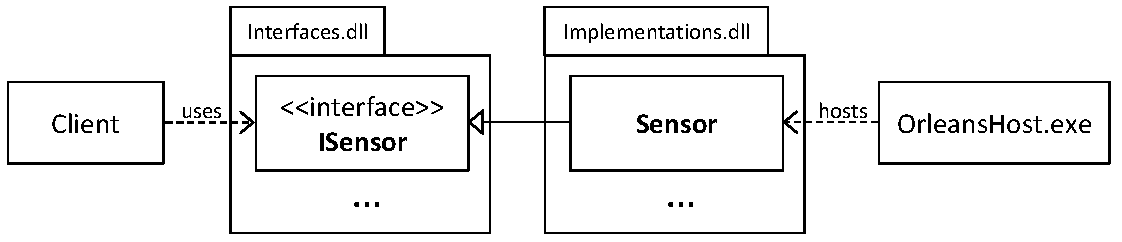
\includegraphics[width=\columnwidth]{orleans-hosting.pdf}%
\caption{Architektur von Anwendungen in Orleans}%
\label{fig:orleans-arch}%
\end{figure}

\subsubsection{Verwendung von Aktoren}

Der erste Schritt um mit einem Aktor interagieren zu können ist per Identität eine Referenz anzufordern. Die Hilfsfunktion \lstinline{GetGrain} gibt als Resultat eine Stellvertreterobjekt für den angeforderten Aktor zurück, dass die Schnittstelle des Aktors implementiert. Es ist nicht erforderlich den Aktor explizit zu Starten oder die tatsächliche physische Adresse herauszufinden. Diese Aufgaben sind Teil der Orleans"=Laufzeitumgebung. In Programm~\ref{prog:orleans-actor-client} ist die Kommunikation mit einem Aktor dargestellt.

\begin{program}[!hbt]
\caption{Verwendung eines Aktors in Orleans}
\label{prog:orleans-actor-client}
\begin{CsCode}
var sensorId = Guid.Parse("eeb48102-c52f-4929-b7b3-da7cce96503f");
var sensor = GrainClient.GrainFactory.GetGrain<ISensor>(sensorId);
for(var i = 0; i < 10; i++)
  await sensor.AddMeasure(random.NextDouble());
Console.WriteLine($"Avg: {/+\textcolor{keywordColor}{await} sensor.GetAverage()+/}");
\end{CsCode}
\end{program}

%the dollar sign in the code above breaks the texniccenter syntax coloring. This invisible dollar escapes from math mode
\iffalse $ \fi

Das vom Klienten verwendete Stellvertreterobjekt wird automatisch von Orleans generiert. Standardmäßig wird der Stellvertreter schon zur Übersetzungszeit erstellt und als Teil der Schnittstellen"=Bibliothek gespeichert. Es wäre aber auch Möglich den Stellvertreter erst zur Laufzeit zu erzeugen.

\subsection{Persistente Aktoren}

Wenn der Zustand eines Aktors nur in Form von Klasseneigenschaften gespeichert ist, wie in Programm~\ref{prog:orleans-actor-impl} gezeigt, so ist dieser nur für die Dauer einer Aktivierung persistent. Sobald der Aktor wegen längerer Inaktivität deaktiviert wird, oder es zu einem Absturz kommt, geht der Zustand verloren. Für manche Daten, vor allem jene die sehr leicht zu berechnen sind, kann diese Form der Speicherung ausreichend sein. Häufig ist es aber auch von Vorteil den Zustand eines Aktors dauerhaft zu persistieren. Man kann natürlich den Zustand selbst in einen persistenten Datenspeicher sicher und immer wieder laden. Das ist aber nicht notwendig, denn Orleans enthält bereits eine Lösung für diese immer wiederkehrende Anforderung. Um den Zustand eines Aktors zu persistieren, sind folgende Schritte erforderlich:

\begin{itemize}
	\item Der Aktor muss von der Klasse \lstinline{Grain<T>} ableiten sein, wobei der Typparameter \lstinline{T} ein Platzhalter für den tatsächlichen Typs des Zustandes ist. Dieser kann entweder ein primitiver Typ sein, oder eine beliebige Klasse.
	\item In der Konfiguration des Aktorsystems muss ein entsprechender Speichermechanismus registriert sein. Es gibt verschiedene bestehende Implementierungen wie \zB Azure Table Storage oder SQL"=Datenbanken. Alternativ ist es auch möglich eine eigene Implementierung zu entwickeln.
	\item Außerdem muss der Aktor mit dem Attribut \lstinline{StorageProvider} annotieren sein, sodass dieser weiß, welcher vorher konfigurierte Speicher verwendet werden soll.
\end{itemize}

In Programm~\ref{prog:orleans-persistent-actor} ist ein Aktor gezeigt, der seinen Zustand persistent speichert. In diesem Fall ist der Zustand in der Klasseneigenschaft \lstinline{State} lediglich eine natürliche Zahl. Änderungen werden erst nach einem Aufruf der Funktion \lstinline{WriteStateAsync} in den persistenten Speicher geschrieben. Ansonsten würde sich der Zustand nur für die aktuelle Aktivierung ändern.

\begin{program}[!hbt]
\caption{Implementierung eines persistenten Aktors in Orleans}
\label{prog:orleans-persistent-actor}
\begin{CsCode}
[StorageProvider(ProviderName="<provider-name>")]
public class PersistentCounter : Grain<int>, IPersistentCounter   {
	public async Task<int> GetCount() => State;
	public async Task Increment() {
		State++;
		await WriteStateAsync();
	}
}
\end{CsCode}
\end{program}

\subsection{Clustering}

Ein Cluster besteht aus einer Menge von Silos, die zu einer Einheit verbunden sind. In diesem Kontext ist mit einem Silo eine Instanz der Orleans"=Laufzeitumgebung gemeint, von denen auch mehrere auf einem einzigen physischen Rechner existieren können. Jeder Silo muss wissen welche anderen Silos ebenfalls Mitglieder des Clusters sind. Die Anzahl der Silos bestimmt nämlich wie der  Wertebereich der Identitäten der Aktoren auf die Silos aufgeteilt ist. Sie müssen sozusagen eine Konsens über die Liste von Mitgliedern finden, damit alle Silos ein global einheitliche Sichtweise haben. Eine Lösung für diese in verteilten Systemen häufig auftretende Problemstellung ist die Verwendung des Paxos"=Algorithmus~\cite{Lamport:1998:PP:279227.279229}. Eine Einschränkung dieses Algorithmus ist jedoch, dass für die Entscheidungsfindung eine Mehrheit der Mitglieder, ein sogenanntes Quorum, notwendig ist. Orleans hingegen setzt auf ein eigens entwickeltes Protokoll, das die Liste der Mitglieder in einer externen tabellenartigen Datenstruktur speichert. Für diese Datenstruktur eignen sich verschiedene Speichersysteme wie \zB  Azure Table Storage oder eine SQL"=Datenbank.

In der Mitgliederliste hat jeder Silo einen eigenen Eintrag, der verschiedene Informationen enthält, wie \zB den aktuellen Zustand. Diese Datenstruktur erfüllt zwei wichtige Aufgaben. Zum einen wissen damit alle Silos welche Teilnehmer der Cluster enthält und zum anderen benötigen auch Klient diese Informationen um sich mit dem Cluster zu verbinden. Die nachfolgende Auflistung gibt einen Überblick über die Funktionsweise des in Orleans umgesetzten Protokolls~\cite{Bernstein2014}:

\begin{itemize}
	\item Jeder Silo trägt sich nach dem Starten in die Mitgliederliste ein.
	\item Die Silos im Cluster überwachen sich gegenseitig durch das periodische Senden von Kontrollnachrichten. Die Identität jedes Aktors wird mit Hilfe eines konsistenten Hashverfahren auf einen zyklischen Wertebereich abgebildet. Damit sind die Silos geordnet und jeder kann eine gewissen Anzahl von zu überwachenden Nachfolgern auswählen.
	\item Wenn mehrere Überwachungsanfragen von Silo $S$ an Silo $T$ fehlschlagen, vermerkt $S$ diesen verdächtigen Vorfall in der Mitgliedertabelle bei Silo $T$.
	\item Übersteigt die Anzahl von verdächtigen Vorfällen innerhalb einer gewissen Periode einen Grenzwert, so deklariert Silo $S$ Silo $T$ als nicht mehr Verfügbar. Anschließend sendet $S$ eine Aufforderung an alle Silos die Mitgliederliste neu zu laden. Wenn alle Silos ihre Mitgliederliste aktualisiert haben, ist Silo $T$ nicht mehr Teil des Clusters.
\end{itemize}

Die Konfiguration eines Clusters ist durch das dynamische Mitgliederprotokoll in Orleans sehr einfach. Ein Silo benötigt einen TCP"=Port für die Kommunikation mit anderen Silos und einen weiteren für die Verbindung zu Klienten. Sowohl bei allen Silos als auch bei den Klienten muss der selbe Speicher für die externe Mitgliederliste definiert sein. Wenn alle Einstellungen korrent konfiguriert sind, können neue Silos einfach zur Laufzeit hinzugefügt oder entfernt werden.

\subsection{Lastverteilung in einem Cluster}

Verwender von Orleans haben nur begrenzten Einfluss auf die Verteilung der Aktivierungen von Aktoren auf die Silos eines Cluster. Ein Grundgedanke von Orleans ist es derartige Entscheidungen in der Laufzeitumgebung zu treffen, um den Verwender zu entlasten. Anstelle Aktoren direkt und mit einem deterministischen Verfahren Silos zuzuordnen, speichert Orleans den Ort einer Aktivierung in einem auf allen Silos verteilten Verzeichnis~\cite[5]{virtualActors}. Durch diese zusätzliche Indirektion hat die Laufzeitumgebung von Orleans mehr Freiheiten die Aktoren zu platzieren und dynamisch umzuverteilen. Wenn ein Klient mit einem Aktor interagieren will, sind dafür zwei Schritte notwendig. Er sendet stellt seine Anfrage an einen beliebigen Knoten im Cluster. Dieser muss zuerst denjenigen Silo auffinden, der die Partition des verteilten Verzeichnisses für den angeforderten Aktor zuständig ist. Dort befindet sich die Information, auf welchem Silo möglicherweise bereits eine Aktivierung läuft. Wenn noch keine Aktivierung vorhanden ist, muss diese erst erzeugt werden. Der zweite Schritt bestehen darin, den Klienten auf den Silo der tatsächlichen Aktivierung weiterzuleiten.

Das Verzeichnis ist als eine verteilte Hashtabelle implementiert, in der jeder Knoten einen anderen Teilbereich des gesamten Wertebereichs verwaltet~\cite{Stoica:2001:CSP:383059.383071}. Sowohl die Identität eines Aktors, aber auch die Identität eines Silos werden mit Hilfe eines konsistenten Hashverfahrens auf den selben zirkulären Wertebereich abgebildet. Durch die Gleichverteilung der Hashfunktion ergibt sich automatisch eine gleichmäßige Verteilung der Identitäten der Aktoren auf alle Silos eines Clusters. Der Vorteil dieses Verfahrens gegenüber klassischer Hashverfahren liegt darin, dass sich bei einer Änderung in der Mitgliederliste im Durchschnitt die Zuordnung von nur $K/n$ Aktoren ändert, wobei $K$ die Größe des Wertebereichs ist und $n$ die Anzahl der Silos. Bei der Zuweisung mit einem normalen Hashverfahren würde sich praktisch die gesamte Zuordnung verändern.

Ein Eintrag in diesem verteilten Verzeichnis beinhaltet die Identität des Aktors und die Adresse des Silos auf dem eine Aktivierung eines Aktor bereits existiert. Wenn noch keine Aktivierung existiert muss eine neue Aktivierung zuerst erzeugt werden. Standardmäßig wird eine Aktivierung auf einem zufällig ausgewählten Silos gestartet. Es gibt aber auch noch weitere Strategien, wie \zB auf dem Silo mit den wenigstens Aktivierungen. In Abbildung ~\ref{fig:orleans-acor-placement} ist noch einmal verdeutlicht, wie Aktoren in Orleans in einem Cluster verteilt werden.

\begin{figure}[!hbt]%
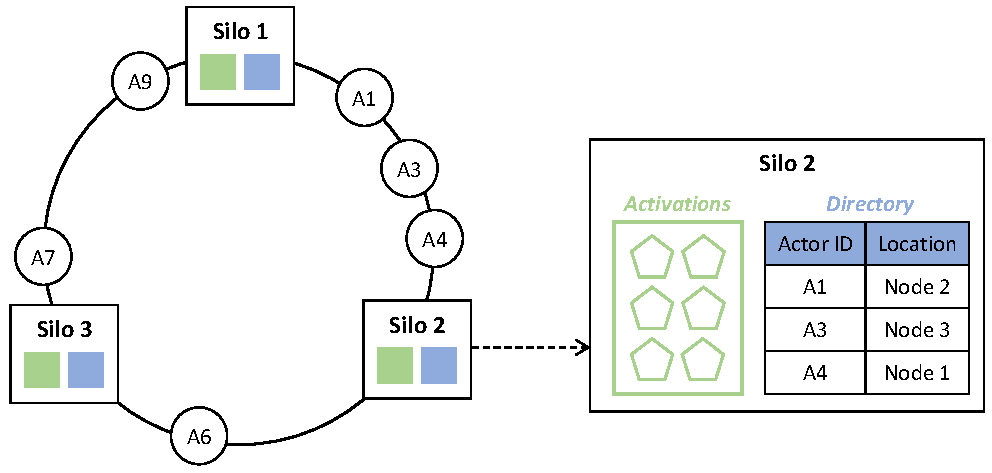
\includegraphics[width=\columnwidth]{orleans-actor-placement.pdf}%
\caption{Bla}%
\label{fig:orleans-acor-placement}%
\end{figure}

Die zusätzliche Indirektion durch das verteilte Verzeichnis macht das Auffinden des Ortes einer Aktivierung zu einer aufwändigen Operation. Aus diesem Grund hält jeder Silo erfolgreich aufgelöste Aktivierungen in einem Zwischenspeicher.

\subsection{Fehlerbehandlung}

Ein Aspekt in dem Orleans wesentlich vom traditionellen Aktorenmodell abweicht, ist die Behandlung von Fehlern. Wie der Abschnitt über Erlang gezeigt hat, ist eine Konsequenz des asynchronen Nachrichtenaustauschs, dass Fehler nicht vom Aufrufer behandelt werden können. Stattdessen muss jemand anderer den an einem möglicherweise entfernten Ort aufgetretenen Fehler behandeln. Dazu ist mit dem Supervisorbaum definiert, welcher Aktoren sich um die Fehler von anderen Aktoren kümmern. Der Supervisor bekommt einfach eine Fehlernachricht und muss über das weitere Vorgehen entscheiden.

Mit dem Programmiermodell von Orleans ist es dem Aufrufer möglich Fehler selbst zu behandeln. Tritt ein Fehler bei einem Funktionsaufruf auf, wird dieser zum Klienten gesendet und dort wieder als gewöhnliche .NET"=Ausnahme geworfen. Die dafür benötigte Logik ist in den von Orleans automatisch generierten Stellvertreterobjekten implementiert. Es ist nicht notwendig Aktoren neu zu starten, weil sie ohnehin beim nächsten Aufruf automatisch neu gestartet werden.

Standardmäßig wird in Orleans eine Nachricht höchstens einmal zugestellt. Der Aufrufer einer Methode bekommt entweder im Erfolgsfall eine Ergebnis zurück, oder wenn die Nachricht verloren ging, eine Zeitüberschreitung die sich als .NET"=Ausnahme manifestiert. Im Fehlerfall ist der Anwender selbst gefordert die Anfrage zu wiederholen. Alternativ kann auch eine automatische Wiederholung von nicht beantworteten Anfragen eingestellt werden. Damit ist es aber möglich, dass die selbe Nachricht mehrfach zugestellt wird. In diesem Fall müssen die aufgerufenen Methoden idempotent sein oder selbst eine mehrfache Zustellung erkennen und ignorieren.

Es ist normalerweise garantiert, dass nur eine Aktivierung eines Aktors zu selben Zeit existiert. Es gibt aber einen Ausnahmefall in dem diese Garantie nicht gilt. Wenn nach einem Ausfall eines Silos zwei Silos noch nicht die selbe Sichtweise auf die Mitgliederliste haben, kann es sein dass beide die Aktivierung eines Aktors anfordern. In diesem Fall existieren zwei Aktivierungen des selben Aktors gleichzeitig. Sobald die Silos die selbe Sichtweise auf die Mitgliederliste haben, wird eine der Aktivierungen terminiert, sodass schlussendlich nur noch eine übrig bleibt. Diese Art der Konsistenz wird als \textit{Eventual Consistency} bezeichnet, weil schlussendlich eine konsistenter Zustand erreicht wird. In Orleans wird also die Verfügbarkeit der Konsistenz vorgezogen. Bei persistenten Aktoren kann das beschriebene Phänomen leicht zu unerwarteten Inkonsistenzen kommen. Wenn beide Aktivierungen den Zustand zur selben Zeit aus dem externen Speicher laden und wieder speichern, geht eine Änderung verloren.

\pagebreak

\section{Aktorenmodell und Microservices}

- Don't start with a monolith
- Actormodel provides good modularization concepts
- No independent deployment? Hot Code Swapping? Most of the time unnecessary complexity. Only for really important components. Upgrade one node after the other
- More efficient communication (no REST/JSON) ...
- Understandable (state diagrams)

\iffalse

Basic Structure:
- Actor Model Basics
- Erlang
- Elixir
- Virtual Actor Pattern
- Orleans
- Conclusion
  - Different Names: Actors, Processes, Grains ... same principles
	- Different Programming models: function vs oo

\fi
\chapter{Ergebnisse und Ausblick}

Das Ziel dieses Kapitels ist es, die bisher betrachteten Konzepte zu reflektieren und Empfehlungen für geeignete Anwendungsgebiete zu geben. In manchen Bereichen stehen diese Konzepte in Konkurrenz zueinander und in anderen wiederum ergänzen sie sich. Es ist auch wichtig zu erkennen, wann eine Technologie unvorteilhaft ist. Für qualifizierte Technologieentscheidungen sind daher Empfehlungen wie die folgenden sehr wertvoll. 

\section{Microservices}

Das Kapitel über Microservices hat sich eingehend der Frage gewidmet, welche Vorteile die Microservices"=Architektur gegenüber einer monolithischen Architektur bietet. Hierbei ist auch klar geworden, dass sich die Vorteile, wie entkoppelte Deployments, ein effizienterer Entwicklungsprozess oder der heterogene Technologieeinsatz, nur für Projekte von bestimmter Komplexität lohnen. Für kleine Projekte und Neuentwicklungen ist die Microservice"=Architektur wenig geeignet. Vielmehr ist hier der Weg der evolutionären Softwarearchitektur zu empfehlen. Dabei wird eine bestehende -- \zB monolithische -- Anwendung sukzessive in eine Microservice"=Architektur umgewandelt. Bis zu einer bestimmten Größe \bzw Komplexität ist die Entwicklung einer monolithischen Anwendung effizienter als eine in Microservices zerlegte Anwendung. Änderungen und neue Funktionen lassen sich in einer monolithischen Architektur viel schneller umsetzen.

Nichtsdestotrotz ist die Microservice"=Architektur derzeit der führende Ansatz für die Entwicklung skalierbarer und robuster Anwendungen. Dabei skaliert dieser Ansatz nicht nur auf technischer sondern auch auf organisatorischer Ebene. Die Verteilung der Verantwortlichkeiten ermöglicht auch bei einer großen Anzahl von Entwicklern noch immer einen reibungslosen Entwicklungsprozess. Aber erst effiziente Bereitstellungsmethoden, wie PaaS, Container \ua, sowie leichtgewichtige Kommunikationsprotokolle haben den Erfolg von Microservices eingeleitet.

\section{Container-Technologien}

In den letzten Jahren hat sich die Virtualisierung durch Container stark weiterentwickelt. Getrieben wurden diese Entwicklungen hauptsächlich von Cloud"=Anbietern, die ein großes Interesse an der Reduzierung ihrer Infrastrukturkosten hatten. Nur mehr für sicherheitskritische Szenarien ist der Einsatz von virtuellen oder gar physischen Maschinen notwendig.

Aus Entwicklersicht hat ein Container alle Funktionen, die auch eine klassische virtuelle Maschine bietet. Ein Service in einem Container kann daher auf alle Technologien zurückgreifen, die das Container"=Betriebssystem unterstützt. Die Vorteile und Risiken von heterogenem Technologieeinsatz wurde bereits ausführlich erläutert.

Sowohl Microservices als auch Container liegt die Philosophie zugrunde, dass sie nur eine Aufgabe erfüllen. Jeder Microservice sollte daher in einem eigenen Container bereitgestellt werden. Die Verwaltung von Anwendungen mit vielen Containern kann aber sehr aufwändig werden. An dieser Stelle ist es meistens notwendig, auf einen Container"=Orchestrierer zurückzugreifen. Dieser verteilt Container automatisch auf eine Menge von Maschinen. Außerdem gehört automatische Skalierung, Fehlerüberwachung und die Verwaltung des Lebenszyklus eines Containers zu den Vorzügen dieser Systeme.

\section{Serverlose Softwarearchitektur}

Function-as-a-Service wirkt wie der nächste logische Schritt in der Evolution von verwalteter Infrastruktur. Verwender sind vollständig von Aufgaben bezüglich Provisionierung und Skalierung von Infrastruktur freigestellt. Es handelt sich bei FaaS um eine produktive, aber relativ unflexible Möglichkeit, Funktionalität bereitzustellen. Mit fehlender Flexibilität ist hier gemeint, dass Entwickler keinen Einfluss darauf haben, wie die FaaS"=Plattform Funktionen betreibt und verteilt. In vielen Szenarien ist aber große Flexibilität gar nicht notwendig. Hier kann FaaS vorteilhaft sein.

In vielen PaaS"=Technologien erfolgt die Kostenabrechnung anhand der Zeit, in denen Ressourcen zur Verfügung standen. Oft werden die Ressourcen aber gar nicht oder nur teilweise genutzt. Bei FaaS erfolgt die Verrechnung nur nach tatsächlich konsumierter Leistung. Gerade am Beginn von neuen Projekten kann dieses verbrauchsbezogene Verrechnungsmodell Kosten einsparen. Bei vorhersehbaren oder speziellen Lastaufkommen können aber optimierte alternative Lösungen die Kosten von FaaS unterbieten.

Die Zeit zwischen der Entwicklung von Funktionen und der tatsächlichen Verfügbarkeit für den Endbenutzer ist bei FaaS herausragend. Entwickler konzentrieren sich nämlich hauptsächlich auf Geschäftslogik und kaum mehr um Infrastrukturaufgaben. Mit nur wenigen Schritten sind die entwickelten Funktionen global, fehlertolerant und skalierbar bereitgestellt.

Das ereignisgesteuerte Programmiermodell von FaaS führt meistens zu einer lose gekoppelten Architektur. Damit ist es relativ unproblematisch, neue Funktionen hinzuzufügen \bzw bestehende zu ersetzen. Die Ereignisse kommen hauptsächlich aus anderen verwalteten Diensten, wie \zB von Datenbanken, Warteschlangen oder Zeitgebern. Auch die Ein"= und Ausgaben haben oft mit verwalteten Diensten zu tun. \Dah FaaS fokussiert sich auf die Integration von verwalteten Diensten und setzt dabei auf bestehende Standardkomponenten. In Systemen, die solche Komponenten bereits intensiv einsetzen, kann FaaS die notwendige Integrationslogik vereinfachen.

Für Anwendungen mit sehr geringen Latenzzeiten scheint FaaS derzeit noch kein geeigneter Ansatz zu sein. Wie in dieser Arbeit gezeigt wurde, wirken sich Kaltstarts signifikant auf die Latenzzeit aus. Außerdem sind viele Ereignisse mit einer Pull"=Strategie implementiert, die natürlich höhere Latenzzeiten als eine Push"=Strategie aufweist.

\section{Aktorenmodell}

Beim Aktorenmodell handelt es sich um ein formales Modell für nebenläufige Berechnungen. Dieser Ansatz eignet sich vor allem für Szenarien, in denen es eine große Anzahl von eigenständigen, gleichzeitig miteinander interagierenden Objekten gibt. Jedes dieser Objekte verarbeitet eingehende Nachrichten ausschließlich sequentiell und stellt somit eine koordinierte Verarbeitung sicher. Es lassen sich viele Softwaresysteme auf intuitive Weise als ein System von Aktoren darstellen. Beispielsweise können Benutzer, Geräte, Sensoren, Warenkörbe eines Onlineshops \usw als Aktor modelliert werden.

Wenn geringe Latenzzeiten für eine Anwendung essentiell sind, kann das Aktorenmodell eine gute Wahl sein. Denn obwohl jeder Aktor seine Nachrichten in einer Warteschlange zwischenspeichert, geschieht die Abarbeitung meistens sehr zeitnah. Es ist ohnehin selten, dass ein Aktor sehr viele Nachrichten verarbeitet. Die Skalierbarkeit des Aktorenmodells resultiert aus den vielen Aktoren, die parallel ihre Nachrichten sequentiell abarbeiten.

Aktoren teilen viele Gemeinsamkeiten mit Microservices. Beide sind relativ kleine Einheiten, die möglichst nur eine einzige Anforderung erfüllen. Sie agieren mit ihrer Umwelt ausschließlich über definierte Nachrichten. Aufgrund der Ähnlichkeit beider Ansätze ist es relativ einfach, aus einem Aktorensystem einzelne Microservices herauszulösen. Im Sinne der evolutionären Softwarearchitektur sollte dies nur bei einem triftigen Grund erfolgen.

Im Kapitel über das Aktorenmodell wurden verschiedene Implementierungen betrachtet. Es gibt aber auch noch weitere in dieser Arbeit nicht behandelte Varianten. Welche davon für eine Anwendung geeigneter ist, lässt sich nicht einfach pauschal beantworten. Aber wie der Vergleich zwischen Erlang und Orleans gezeigt hat, unterscheiden sich diese Varianten doch sehr wesentlich. Erlang bietet die größten Eingriffsmöglichkeiten, erfordert daher aber auch viel Implementierungsaufwand. Im Gegensatz dazu ist der Einstieg in Technologien wie Orleans etwas leichter. Es kann aber der Zeitpunkt kommen, an dem Orleans zu viele Entscheidungen für den Entwickler getroffen hat und die Flexibilität von Erlang wünschenswert wäre. Ebenfalls nicht zu vernachlässigen ist, dass Orleans auf der weitverbreiteten .NET"=Plattform aufsetzt. So können bestehende .NET"=Bibliotheken mit Orleans wiederverwendet werden.

Das Aktorenmodell lässt sich mit unterschiedlichen Programmierparadigmen implementieren. Die funktionale Programmiersprache Erlang verfolgt natürlicherweise einen funktionalen Ansatz. Im Gegensatz dazu hat Orleans mit der Objektorientierung ein Paradigma herangezogen, das vielen Entwicklern vertraut ist. Oft wirkt der funktionale Ansatz natürlicher. Beispielsweise sind die Zustände eines Aktors sehr intuitiv als Funktionen modelliert. Mit Hilfe von Mustervergleichen kann auch die Nachrichtenselektion prägnant formuliert werden. In objektorientierten Varianten ist es nicht sofort ersichtlich, in welchem Zustand sich ein Aktor befindet. Außerdem muss jede Methode eines Aktors den aktuellen Zustand überprüfen, was unweigerlich zu viel Entscheidungslogik führt. Aber diese beiden Ansätze unterscheiden sich nur äußerlich, funktional sind sie isomorph.

Viele Applikationen verwenden eine relationale Datenbank als externes Speichermedium. Mit persistenten Aktoren, so wie in Orleans, können Aktoren ihren Zustand automatisch mit einem externen Speicher synchronisieren. Es ist also nicht notwendig, die Daten noch separat in einer Datenbank zu speichern. Somit ist es auch nicht notwendig, eine Abbildung der objektorientierten Daten auf ein häufig relationales Datenmodell abzubilden.

Das Aktorenmodell war lange Zeit etwas in Vergessenheit geraten, obwohl schon von Beginn an brauchbare Implementierungen, wie \zB Erlang existierten. Für skalierbare und robuste Anwendungen ist ein verteiltes Programmiermodell unumgänglich. Mit dem Aufstieg von Cloud"=Computing und verteilter Programmierung stieg auch das Interesse an Aktorsystemen wieder. Festzumachen ist diese Erkenntnis an den vielen neuen Implementierungen, die in den letzten Jahren erschienen sind. In Zukunft könnte das Aktorenmodell also mehr Bedeutung denn je bekommen.

%%%----------------------------------------------------------
\appendix                                            % Anhang 
%%%----------------------------------------------------------

% Empty

%%%----------------------------------------------------------
\MakeBibliography                        % Quellenverzeichnis
%%%----------------------------------------------------------

%%% Messbox zur Druckkontrolle ------------------------------
%\chapter*{Messbox zur Druckkontrolle}



\begin{center}
{\Large --- Druckgröße kontrollieren! ---}

\bigskip

\Messbox{100}{50} % Angabe der Breite/Hoehe in mm

\bigskip

{\Large --- Diese Seite nach dem Druck entfernen! ---}

\end{center}



%%%----------------------------------------------------------
\end{document}
%%%----------------------------------------------------------